\documentclass{article}
\usepackage[utf8]{inputenc}
\usepackage{fullpage}
\usepackage[backend=biber,style=apa,backref=true]{biblatex}
\usepackage{listings}
\usepackage[capposition=top]{floatrow}
\newcommand{\ra}[1]{\renewcommand{\arraystretch}{#1}}

\usepackage{xcolor}
\colorlet{punct}{red!60!black}
\definecolor{background}{HTML}{EEEEEE}
\definecolor{delim}{RGB}{20,105,176}
\colorlet{numb}{magenta!60!black}

\lstdefinelanguage{json}{
    basicstyle=\normalfont\ttfamily,
    numbers=left,
    numberstyle=\scriptsize,
    stepnumber=1,
    numbersep=8pt,
    showstringspaces=false,
    breaklines=true,
    frame=lines,
    backgroundcolor=\color{background},
    literate=
     *{0}{{{\color{numb}0}}}{1}
      {1}{{{\color{numb}1}}}{1}
      {2}{{{\color{numb}2}}}{1}
      {3}{{{\color{numb}3}}}{1}
      {4}{{{\color{numb}4}}}{1}
      {5}{{{\color{numb}5}}}{1}
      {6}{{{\color{numb}6}}}{1}
      {7}{{{\color{numb}7}}}{1}
      {8}{{{\color{numb}8}}}{1}
      {9}{{{\color{numb}9}}}{1}
      {:}{{{\color{punct}{:}}}}{1}
      {,}{{{\color{punct}{,}}}}{1}
      {\{}{{{\color{delim}{\{}}}}{1}
      {\}}{{{\color{delim}{\}}}}}{1}
      {[}{{{\color{delim}{[}}}}{1}
      {]}{{{\color{delim}{]}}}}{1},
}


\usepackage{url}
\usepackage{graphicx}
\graphicspath{./figs}
\usepackage{amsmath}
\usepackage{hyperref}
\hypersetup{colorlinks=true, citecolor=blue}

%for including wordcount in file
\immediate\write18{texcount -template="{word} words in main body, excluding headers and bibliography." \jobname.tex -out=\jobname.sum}
\usepackage{verbatim}
\usepackage{setspace}
\usepackage{booktabs}
\usepackage{lscape}
\doublespacing
\newcommand\wordcount{\verbatiminput{\jobname.sum}}


\author{George Tyler}
\date{\today}

\addbibresource{diss.bib}
\begin{document}

\title{Social Media, Risk Perception, and Social Distancing: \\ Evidence from 15.3 Million Geolocated Tweets}

\maketitle

\abstract{Does social media predict risk-taking behaviour? I investigate this question in the context of COVID-19 by exploiting a large panel of tweets. Using inferred and explicit geolocation data embedded in the tweets, I study the extent to which public expressions of sentiment influence social distancing, as measured by GPS-located smartphone data. Using a two-way fixed-effects design over two different methods of measuring sentiment, I find a fair amount of consistent evidence for a correlation between sentiment and community mobility, but the results are not robust to alternative specifications. Implications and areas for further research are discussed. The dissertation also contains an primer of text analysis in economics.}
\wordcount

\tableofcontents

\section{Introduction}
\subsection{Overview}\label{overview}
The early stages of the COVID-19 pandemic saw an unprecedented shift in behaviour for most citizens of the United States. In a short period of time, a large number changed their habits of working, socialising, and travelling. They did so both as a result of government restrictions in the form of non-pharmaceutical interventions (NPIs) and as a private response to the spread of the pandemic. Economists have taken interest in how citizens formed these behaviour changes, and the role that beliefs and risk attitudes played in determining the response to public policy. A new way to measure belief formation and public sentiment is with social media, an increasingly common platform for expression of opinion. It is plausible that those who express more risk-averse sentiment towards COVID online will be inclined to respond in a stricter fashion to social distancing and other public health regulations. In this dissertation, I study the impact of local expressions of risk attitude on public behaviour in the early months of the pandemic. Specifically, I study whether a measure of risk-averse sentiment on Twitter is linked to increased social distancing behaviour at the county/week level. 

This dissertation contributes to two strands of the recent economics literature on the COVID-19 pandemic. First, it investigates the relationship between partisanship and risk preference. Previous papers posit that political preference influences social distancing through risk preference; I contend that \textit{local} risk preference is a separate factor to political partisanship, and has an independent impact on social distancing. More broadly, the paper investigates the relationship between risk preference and economic behaviour, and presents a novel example of economic inference from social media using text analysis. 


A key vector for expressing sentiment is social media, with Twitter and Facebook's suite of products\footnote{Facebook, Facebook Messenger, Instagram, and WhatsApp} being the most widely-adopted, each platform having over 80 million monthly active users in the US. A survey by the Pew Research Foundation indicates that 22\% of US adults use Twitter, with 42\% of these using it on a daily basis \parencite{perrinShareAdultsUsing2019}. On Twitter, users can share their own text, with the option to link to a website; alternatively, they can `retweet' another user's text or link. Users can also use `hashtags' in their tweet, which connects their tweet to a particular topic. If the user has allowed it, Twitter also records the location of the tweet; and it is also possible for the user to set their location on their profile. In this way, it is possible to create a panel of geographically-located tweets about a particular topic. 

I exploit GeoCov19 \parencite{qaziGeoCoV19DatasetHundreds2020a}, a dataset of 524 million geolocated tweets, to measure the local public sentiment on COVID in the US. The tweets cover the period from 1st February to 1st May, the period I focus on. The particular subset of the data I use contains 33.36 million tweets in total; a small subset are exactly geolocated (the user has provided a GPS location), while most are inferred from the location tab in the user's profile. The tweets were collected using the Twitter Streaming API, querying for tweets containing any of a list of 800 COVID-related keywords. I also use anonymous smartphone location data, collected by the company SafeGraph, as a measure of the extent of social distancing in an area. I present two measures of social distancing at county level: first, the median minutes spent at home during 8am-6pm; second, the proportion of measured devices that stayed at home all day \parencite{safegraphinc.SocialDistancingMetrics2020}. Demographic controls are also acquired and presented from the American Community Survey and the 2010 US census. 

I use dictionary-based text analysis to assess the level of risk sentiment in a tweet. More sophisticated methods of text analysis like latent factor modelling are discussed in the Methods section. In the absence of a lexicon of risk preference, the NRC Emotion Lexicon \parencite{mohammadCrowdsourcingWordEmotion2013} is used. This is a widely-used mapping of English words to eight basic emotions (anger, fear, anticipation, trust, surprise, sadness, joy, and disgust). Starting from a set of tweets that mention COVID, I assign tweets containing fear-associated words to a risk-averse sentiment. The base unit of analysis is the county-week; as such, I measure the proportion of tweets that contain fearful language in each county and week. 

It is plausible that social media is a valid measure for risk appetite. The intuition is that the textual content of a social media post broadly reflects the poster's current opinion of a topic: for example, in response to the first confirmed US COVID death on February 26th, a user might express fearful sentiment, or a neutral sentiment. This opinion of the topic, particularly their level of fear, maps to a user's broader expectations about the course of the pandemic: while other emotions like joy, anticipation, and trust may rely on the context of the discussion, expressions of fear are plausibly consistent in mapping to risk-averse sentiment. When restrictions are implemented, users who initially formed pessimistic expectations may be more inclined to adhere more to them than a user who formed optimistic or netural expectations. The key aspect to the data is that the Twitter conversations provide a real-time insight into local sentiment as NPIs are implemented; this sentiment changes both in response to current, local experience \textit{and} broader partisan interpretations of current events.

The primary econometric specification is a panel model with county and week fixed effects;
\begin{equation}
  SD_{ct} = \mathbf{B}_{ct} \mathbf{S} + \Theta_{ct} \mathbf{C} + \gamma_c + \delta_w
\end{equation}
where \(SD_{ct}\) is a vector of social distancing metrics, \(\mathbf{B}_{ct}  \mathbf{S}\) is a matrix of two risk perception measures (i.e. the proportion of total tweets containing fearful language and the number of tweets), \(\Theta_{ct} \mathbf{C}\) a matrix of time-varying confounders (the COVID deaths and two policy variables), and \(\gamma_c + \delta_w\) county and week-level fixed effects. 


This research contributes to the recent economics literature seeking to explain the disparities in social distancing in the early stages of the pandemic in the US. In particular, partisanship has been shown to be a significant factor on the practice of social distancing: \textcite{allcottPolarizationPublicHealth2020,barriosRiskPerceptionLens2020,painterPoliticalBeliefsAffect2020} show that areas with more Republicans engaged in less social distancing, are associated with lower perceptions of risk of the pandemic, and exhibited less remote transactions. \textcite{simonovPersuasiveEffectFox2020,ananyevSafestTimeFly2020} also measure the causal effect of the right-wing Fox News network on social distancing during the pandemic. This paper builds on \textcite{barriosRiskPerceptionLens2020} in particular, which shows that online risk perception is predicted by Trump voter share: by measuring risk perception with a high-frequency geolocated dataset, my approach controls for political alignment and assesses the effect of risk perceptions on their own. In essence, I measure expressions of sentiment regarding COVID risk, and given this data I ask whether local risk sentiment predicts social distancing behaviour beyond political affilitation. Second, this research relates to the recent economics literature around heterogeneous-agent epidemiological models, which endogenise individual behaviour -- including social distancing -- into the effective reproductive number \(R(t)\). These recent models, such as \textcite{acemogluTestingVoluntarySocial2020,brotherhoodEconomicModelCOVID192020,eichenbaumMacroeconomicsEpidemics2020}, assume that preferences over risk are predictive of social distancing behaviour; this paper looks to empirically confirm this key assumption.

%This paper is particularly close to two research papers, This dissertation takes a similar approach, but uses Twitter as a news source instead. More broadly, this dissertation contributes to the literature on the effects of misinformation and political affiliation on public behaviour.

This dissertation also contributes to the rapidly-expanding field of text analysis in economics, and presents an example of how the rich sentiment data encoded in social media communication can inform insights into public behaviour. This topic is particularly mature in finance -- where sentiment data from public company documents, news media, and social media have been shown to predict stock market reactions \parencite{bollenTwitterMoodPredicts2011} -- and monetary economics, where central bank statements, coded according to their attitude to inflation, predict fluctuations in Treasury securities \parencite{luccaMeasuringCentralBank2009,gentzkowTextData2019}. On the topic of empirical economics, this paper takes a similar approach -- by using online data to predict local sentiment -- as \textcite{stephens-davidowitzCostRacialAnimus2014}, which uses Google search data to proxy an area's racial animus, and uses this to estimate the Obama vote share. I use geolocated Twitter sentiment to proxy the local attitude to COVID in a given week, and test to see if this predicts social distancing practice. 

The argument of the dissertation rests on the following assumptions: first, that social media data is a valid proxy for local risk appetite, and that fear-associated language in COVID-related tweets is an effective estimator of the risk appetite encoded in the tweet. It is also important to note a possible selection effect in the dataset: tweets about COVID may attract a greater level of fear-related language and not reflect an individual's true opinion about social distancing and other preventative measures. I address these assumptions and drawbacks and discuss methods to alleviate them in the Results section.


\section{Literature Review}
\subsection{Text analysis, sentiment mining, and social media in Economics}\label{sentmining}
Ultimately, text is the most popular medium for encoding and recording information. As such, it is the medium for a very large amount of data which could be useful to economic research. The limiting factor to text has been the fact that this information is recorded in a noisy, high-dimensional format; however, recent advances in processing techniques have made it possible to extract the relevant information from text. This process is covered in detail in chapter \ref{textan}; this section reviews the previous applications of sentiment mining in economic research, putting the dictionary-based sentiment mining used in this dissertation in context.

Broadly speaking, sentiment is the disposition of an entity (either an individual or a collective) towards a topic \parencite{algabaEconometricsMeetsSentiment2020}. This disposition has a \textit{polarity}: in the general sense, this corresponds to whether the disposition is positive or negative, but can also reflect domain-specific concepts like Dovish/Hawkish \parencite{picaultWordsAreNot2017} or Democrat/Republican \parencite{gentzkowWhatDrivesMedia2010}. In this way, polarity defines the qualitative notion of disposition as a quantitative measure; this process is described in detail in section \ref{textan}. 

For economists, quantitatively defining sentiment helps to measure economic decision-making: sentiments in personal communications might convey information about the author's expectations and preferences, and sentiments expressed in instituational communications like company filings and news reports might convey information about fundamental economic factors. The concept of polarity is particularly suited to measuring and predicting the impact of confidence in financial markets and other macroeconomic entities; as such, sentiment analysis is a particularly well-established tool in finance research. \textcite{tetlockGivingContentInvestor2007a,antweilerAllThatTalk2004} are prominent examples: both use sentiment polarity as a proxy for investor confidence, analysing news articles and internet message boards respectively. A closely-related application is measuring latent sentiment in the population. For example, \textcite{bakerMeasuringEconomicPolicy2016} show that uncertainty about fiscal, regulatory, and monetary policy has a significant impact on economic activity, and measure this uncertainty by creating an index of the sentiment expressed in newspaper articles. 

Economists have also causally linked sentiment expressed in texts to observed behaviours. \textcite{stephens-davidowitzCostRacialAnimus2014}\footnote{See section \ref{overview} for summary.} is a prominent example of linking county-level variation in sentiment to behaviour, as are \textcite{choiPredictingPresentGoogle2012,saizProxyingUnobservableVariables2013}. \textcite{ginsbergDetectingInfluenzaEpidemics2009} does not measure sentiment, but is one of many examples which use Google searches for influenza symptoms to predict local outbreaks of disease; this dissertation extends this project by treating sentiment as a local-level health indicator. 

We have seen that Google searches are a relatively popular measure of economic sentiment. To a lesser extent, social media has also been used as an indicator for sentiment, particularly in finance. Similar to the empirical strategy of this dissertation, \textcite{affusoSocialMediaSentiment2019} uses the sentiment of geolocated Tweets to measure investor sentiment in different regions; \textcite{bollenTwitterMoodPredicts2011} is a particularly widely-cited example of using Twitter sentiment to predict stock market returns. \textcite{daasSocialMediaSentiment2014} connects Twitter and Facebook sentiment data to Dutch consumer confidence indices, and \textcite{mullerFanningFlamesHate2020} uses geolocated Facebook posts to construct a measure of anti-refugee sentiment, which strongly predicts hate crimes. Finally, \textcite{gorodnichenkoSocialMediaSentiment2018} finds that geolocated tweets about Brexit are a strong predictor of Leave vote-share.

In conclusion, sentiments embedded in social media and other forms of text are a powerful tool in uncovering the determinants of individual behaviour. This dissertation asserts that Twitter sentiment can predict social distancing behaviour: the next section reviews the economic literature on the dynamics and determinants of COVID-19 related behaviour.
\subsection{COVID-19: Individual and demographic determinants of social distancing behaviour}
The primary aim of this dissertation is to investigate the role of anxiety and risk preference in determining social distancing behaviour. There has been a large quantity of work done to investigate the determinants of social distancing, both on an empirical basis and a modelling basis. To inform my econometric specification, it is necessary to account for all possible determinants and causal pathways around risky COVID behaviour. As such, the next two sections summarise the literature on behavioural determinants, starting by addressing the empirical work.

\textcite{glaeserHowMuchDoes2020} documents the variations in SafeGraph mobility across the United States and estimates the effect of mobility reduction in moderating COVID spread. They find that mobility reduction significantly decreases COVID cases, and that the strength of the effect is heterogeneous across different locations. They find a clear importance of mobility reduction to reducing COVID spread. Several factors affect the ability to reduce mobility, and often these differentiate across income. For example, \textcite{wrightPovertyEconomicDislocation2020} shows that areas with low economic endowments complied less with stay-at-home orders, and a one-time cash transfer significantly increased social distancing in these areas. Another factor affecting the ability to socially distance is internet access: \textcite{chiouSocialDistancingInternet2020} show that high-speed internet access accounts for much of the income effect on mobility changes. The correlation between income and internet access shows that ability to self-isolate not only depends on the sector of employment, but also the ability to work remotely in general. \textcite{fanHeterogeneousActionsBeliefs2020} finds systemic differences in SafeGraph-measured mobility along lines of gender, income, and political affiliation at the county level; they also find significant spatial heterogeneity in beliefs and preferences about COVID-19.

A central issue to the dissertation is whether observed mobility changes are a result of policy or a function of individual decisions. The general consensus in the economics literature is that mobility changes pre-date stay-at-home orders, meaning that they are largely attributable to individual responses. Establishing this is a key factor in the identification of fear as a significant factor: since individual responses are important to mobility, it is important to understand and measure the drivers of individual mobility preferences, like anxiety.

\textcite{goolsbeeFearLockdownDiversion2021} is one of a number of papers that addresses the question of mobility as a function of policy or individual action, and is also a broader overview of the empirical factors of social distancing behaviour. They isolate the difference between \textit{fear-driven} voluntary social distancing and policy-driven social distancing by using SafeGraph footfall data on businesses close to a jurisdictional border, where there is policy variation across the border. They find that legal orders only account for a small share of changes in footfall, indicating that most social distancing was in response to \textit{individual} fear. They connect social distancing practice to fear specifically, as the drop in footfall is strongly correlated with local COVID deaths, and increases with the previous busyness of the establishment. In other words, consumers respond to experiencing the \textit{local} impact of COVID, and in consequence avoid places which are perceived to be high-density. \textcite{maloneyDeterminantsSocialDistancing2020} uses Google mobility data for the United States to support the conclusion that voluntary distancing accounted for most of the changes in mobility, though (as would be expected) policy orders do have a smaller but still significant impact. They find that the results are consistent across all but the lowest income group, where COVID-risky jobs are concentrated. 

The interaction between political affiliation and social distancing in the United States is a complex and important factor. Donald Trump initially downplayed the seriousness of the virus and subsequently the imposition of restrictions was made a partisan issue. \textcite{bacciniExplainingGovernorsResponse2021} found that during March 2020 Democratic state governors were 50\% more likely to impose a stay-at-home order, and they did so more quickly in response to cases above a certain threshold\footnote{They control for disease spread by including deaths in the state as a covariate in their OLS specification.}.  In addition to affecting the likelihood  of a stay-at-home order, it has also been shown that political affiliation affects voluntary decisions to socially distance.  \textcite{barriosRiskPerceptionLens2020} is an example of this, investigating individual risk perception and social distancing from a partisan standpoint, written in early to mid-March. Using Google searches for COVID as a proxy for risk perception, they find that these Google searches decline strongly in counties that voted Trump in the 2016 election. They also find that Trump counties exhibit a muted mobility change in response to COVID cases, and comply less with stay-at-home orders. \textcite{painterPoliticalBeliefsAffect2020} also documents this result. \textcite{allcottPolarizationPublicHealth2020} shows that in addition to observed risk and policy, partisanship plays an important role in driving distancing behaviour. They also show through a survey that beliefs about the likelihood of contracting COVID are divided along partisan lines\footnote{This result is generalised by \textcite{pastorPoliticalCyclesStock2020}, who find that Democrats are more risk averse than Republicans.}.  Another aspect to the partisanship divide in distancing is exposure to COVID-sceptical media. \textcite{simonovPersuasiveEffectFox2020,ananyevSafestTimeFly2020} use the same identification strategy, exploiting variation of the position of COVID-skeptical Fox News on the TV dial to conclude that areas with greater exposure to Fox have a muted change in mobility. \textcite{bursztynMisinformationPandemic2020} also uses Fox to show that exposure to COVID-skeptical content decreases risk perception: in late February 2020, viewers of COVID-downplaying \textit{Hannity} changed their mobility later than viewers of a more cautious show on the same network. This research on partisanship and media makes clear several salient points. First, distancing behaviour varied markedly along partisan lines during February and March. Second, the behaviour change was a function of individual beliefs about COVID risk; third, media consumption \textit{in addition to pure partisanship} directly affected these risk beliefs. This body of research shows, then, that political partisanship colours risk perceptions and affects behavioural choices. However, risk perceptions are moderated not only by political beliefs but also by media consumption and other confounding factors like occupation, income, and health risk level. Individual risk perception is important on its own standing and depends on separate local factors as well as partisanship; with this in mind, this dissertation measures and investigates the impact of risk perception \textit{in the abstract} in determining mobility. 

More general research has also been done on health behaviours in the context of the COVID-19 pandemic, which does not include mobility as an observed outcome; rather, these papers identify individual-level determinants of pandemic-related health behaviour. First, \textcite{mullerEconomicPreferencesCompliance2021} uses a survey to elicit preferences over risk, time, trust, and honesty; this is linked to self-reported policy compliance (stay-at-home behaviour, social distancing, and testing), perception of the crisis (panic buying and reported fear of COVID-19), and pre-pandemic social altrusim (fare-dodging, agreement for compulsory measles vaccines). They find that risk aversion, patience, and social responsibility predicts greater social compliance and stay-at-home behaviour, and observe that individuals exhibiting present bias engage in more panic buying. They also find that risk tolerance significantly decreases a subject's reported fear of COVID-19. Another survey-based study is \textcite{thunstromTestingCOVID19Willful2021}. The authors report that fear for one's own health, extraversion, proclivity for policy compliance, and age are primary determinants of whether respondents would attend a costly COVID test. \textcite{brisceseExpectationsReferencePoints2020} also study determinants of policy compliance, and find that expectations about policies serve as a reference point for future compliance efforts. Respondents are less likely to comply with a stay-at-home order if the announced duration is longer than expected, and individuals grow more impatient over time. Finally, \textcite{zettlerRolePersonalityCOVID19forthcoming} finds that individual perceptions in the form of personality traits affect reported compliance behaviours: they find that prosocial traits are a significant predictor of compliant health behaviour\footnote{See also, e.g. \textcite{herrmannAntisocialPunishmentSocieties2008,almasCutthroatCapitalismCuddly2019}}.

Past research in health economics has also addressed the determinants and motivations of health behaviours. First, individual risk preferences matter: \textcite{andersonPredictingHealthBehaviors2008} measures risk preference and health behaviour on a large scale with a lottery choice experiment and survey, finding that risk aversion has a negative association with risky health behaviours like smoking and drinking\footnote{See also, e.g. \textcite{dohmenIndividualRiskAttitudes2011}.}. Second, time preferences matter for determining health behaviour: \textcite{chapmanTimePreferencesPreventive1999} observe in a randomised trial that individuals with lower discount rates with respect to money and health are more likely to take up a free influenza vaccine, with \textcite{harrisonIndividualDiscountRates2010,chessonDiscountRatesRisky2006} reaching equivalent results for smoking and risky sexual behaviour respectively\footnote{See also, e.g.  \textcite{dellavignaPayingNotGo2006,sutterImpatienceUncertaintyExperimental2013,stutzerLimitedSelfcontrolObesity2016,schilbachAlcoholSelfControlField2019}.}. Finally, personality traits can be a determinant of health behaviour: \textcite{rustichiniIntegrationPersonalityTheory2016} find that personality traits and indiviudal preferences are strongly related and predict health behaviours\footnote{See also, e.g. \textcite{booth-kewleyAssociationsMajorDomains1994,strickhouserDoesPersonalityPredict2017}.}.

We have established that several dimensions of individual preference predict social distancing behaviours. There is also some substantial evidence supporting the notion that these preferences vary by region. \textcite{falkGlobalEvidenceEconomic2018} conducted the `Global Preference Survey' of time and risk preference, altruism, and trust over 80,000 people in 76 countries. They found heterogeneity across countries, and even greater within-country heterogeneity. The heterogeneity in preferences tracked with individual characteristics like age and gender, but a substantial proportion of the variation is attributed purely to a region effect, perhaps in the form of culture and bio-geographic variables. As mentioned above, \textcite{fanHeterogeneousActionsBeliefs2020} also supports the notion of spatial heterogeneity, documenting county-level substantial variation in preferences and COVID-related beliefs.

In summary, the general health economics literature and COVID-related work has established that time preferences, risk preferences, pro-social tendencies, and fear of COVID are strong individual determinants of pandemic compliance behaviours. Additionally, there is strong evidence for spatial heterogeneity in these individual preferences and traits. This last point in particular is key for the identification of the empirical specification, since I argue that the research on spatial heterogeneity of preferences allows for an empirical design that measures individual characteristics on the aggregate level. 

\subsection{COVID-19: Models of risk perception and social distancing} 
At the outbreak of the pandemic, many economists augmented the standard epidemiological `Susceptible-Infected-Recovered' (SIR) models with economics-derived models of human behaviour. \textcite{murrayEpidemiologyTimeNeed2020}, writing as an epidemiologist, identifies 
\subsubsection{Standard SIR model}
\textcite{kermackContributionMathematicalTheory1927} introduced the SIR model and it remains the basis for most modern epidemiological models; this explanation follows \textcite{averyEconomistGuideEpidemiology2020}. Each member of the population can be in one of three `Susceptible, Infected, Recovered' states; therefore, at each time period we have

\begin{equation}\label{SIRstates}
    S(t) + I(t) + R(t) = 1
\end{equation}
, where the population is normalized to 1. A susceptible individual can only move to the infected state through contact with an infected individual, and an infected individual can only move to the recovered state. The recovered state, in the base version, includes \textit{both} those who have recovered and those who have died: they share the key characteristics of being noninfectious and not susceptible to future infection. Three key parameters govern the rate of transitions between these states: \(\gamma\), the recovery rate, represents the probability per unit time for an individual to move from Infected to Recovered; \(R_0\), the basic reproductive number, is the ``number of people an infectious person would infect over the course of their disease in a fully susceptible population'' \parencite[81]{averyEconomistGuideEpidemiology2020}. \(R_0\) therefore stands in an inverse relationship with the recovery rate: \(R_0 = \beta / \gamma\), where \(\beta\) is the expected number of contacts an individual makes per unit time in normal circumstances. Assuming that the individual infects every contact, the states evolve according to 

\begin{align}
    \dot{S}(t)&= -S(t)I(t)R_0 \gamma \\
    \dot{I}(t)&= S(t)I(t)R_0 \gamma - \gamma I(t) \\
    \dot{R}(t)&= \gamma I(t)
\end{align}
. For epidemiologists, then, \(R_0\) is seen as a `compound parameter' of both the virus' natural infectivity\footnote{Which itself is governed by the expected length of contagiousness \(\frac{1}{\gamma}\) and the transmissibility, which we assume to be 1.} and the expected number of in-person interactions during pre-pandemic life \parencite[84]{averyEconomistGuideEpidemiology2020}: government policies and behaviour change therefore have the effect of reducing the \(R_0\) parameter to some variable \(R^t_0\). This gives rise to the key aim of `flattening the curve': achieving a state where -- given the current susceptible fraction of the population -- the expected number of people that a contagious individual infects over the course of their illness is below 1:
\begin{equation}
    R_t \equiv R^t_0 S(t) < 1
\end{equation}. \(R_t\) is known as the effective reproductive number.

\textcite{averyEconomistGuideEpidemiology2020} sorts the contributions of economic research to the basic SIR model into three basic categories: pointing out the endogeneity of the reproductive number, adapting the model to heterogeneity of different subpopulations, and adapting SIR models to policy-relevant issues like social distancing compliance. I now set out the insights that model-based COVID economic research gives to the topic in this dissertation: the relationship between risk preferences, local demographic characteristics, and social distancing behaviour.


\subsubsection{Models of endogenous social distancing}
In the base SIR model, \(R^t_0\) is endogenous, since individuals adjust their exposure to others in response to the state of the epidemic. A priority for this dissertation is to establish the characteristics and determinants of social distancing; a large body of literature has emerged in economics discussing this issue. 

\textcite{toxvaerdEquilibriumSocialDistancing2020} models individuals as making non-cooperative, forward-looking decisions to engage in costly social distancing by solving a tradeoff against beneficial social behaviour and the risk of infection. Toxvaerd finds that equilibrium social distancing depends on the threshold infection probability, which is determined by the aggregate disease prevalence; this entails that individuals react to higher prevalence by distancing more, mitigating the flow rate between \(S(t)\) and \(I(t)\). In this model, individuals assess the value of becoming infected as equal to the expected discounted lifetime utility of being in the infected state. The model considers a homogenous population and so does not take demographics into account.

\textcite{farboodiInternalExternalEffects2020} also models the tradeoff of exposure against health risks. Using the SafeGraph dataset, they find that social activity levels fall before imposition of mandatory measures. This yields their key observation: desire to avoid illness is a key determinant of social distancing, meaning that there is a strong laissez-faire reduction in social activity. This cost-response reduction produces the majority of social distancing behaviour, but not enough for optimal pathogen suppression; as such, social distancing orders are recommended. They implement quadratic matching with random search, introduced in \textcite{diamondEquilibriumAnalysisSearch1979}, to model social interactions. Individuals are split into the S, I, R states, where the level of chosen social activity is the same among all individuals in that state. Disease transmission is therefore a function of \(\beta\), the number in the susceptible and infectious states, and the social activity level of each of those states. Individuals choose their level of social activity, taking the external social activity level and the number of infected as a given. The model, however, abstracts from subpopulation heterogeneity.

\textcite{eichenbaumMacroeconomicsEpidemics2020} also point out that exposure comes either from purchasing consumption goods, from working, and from random interactions such as touching surfaces: this shows the importance of income and mode of work for disease transmission. 

\textcite{chernozhukovCausalImpactMasks2021} estimate a structural equations model, which incorporates voluntary social distancing into a causal framework. This framework decomposes the change in COVID caseload into three drivers: direct effects of policies (e.g. mask mandates), behaviour changes due to policies (e.g. stay-at-home-orders), and individual behaviour changes. In their model, individuals respond to global information -- which is represented by month dummies -- and they respond to local information -- which is represented by the local growth rate and total cases. In other words, they take information to be broadly equivalent to lagged health outcomes. Individual-level distancing behaviours are a function of policies, information, and observed confounders. These observed confounders are at the state level and include the demographic characteristics of population, area, unemployment and poverty rates, percentage of people at risk of illness, and governor's party. Their empirical estimation shows that log case growth (at national and county level), stay-at-home orders, and business closure policies have a significant effect on mobility; they find that including case growth in the specification is a moderately better proxy for information than deaths growth. Finally, they find additional evidence that individuals respond voluntarily, in response to information about COVID, rather than as a forced response to policies.


\subsubsection{Subpopulation heterogeneity}
An important contribution that economists made was to incorporate multi-population SIR models. By including separate populations, it is possible to account for the significant heterogeneity in risk with respect to age. In respect of the social distancing risk decision, this variation in the cost of infection is theorised to generate a disparate response in different age brackets, in addition to the usual demographic and occupational variation in mobilty patterns with age. A key component of multi-group SIR models is the expansion of \(R_t\) from a single population average to a matrix with a measure of \(R_t\) for the interactions between subpopulations. In theory, this allows for policies to be targeted at a local and risk-group level; however, in practice this policy approach has not in general been implemented. \textcite{faveroRestartingEconomySaving2020} calibrate an SIR model with nine age brackets and three occupation sectors. In this setting, the decision to risk exposure is a function of the actual probability of infection, the perceived importance of the activity, and the perceived cost of infection. They find that perceived cost is an important factor to reduce risky behaviour. Another multi-population model is \textcite{acemogluOptimalTargetedLockdowns2020}, which advocates for targeted age-dependent policies as a significant utility increase over blanket policies. In an optimal-control model with state variables \(S\), \(I\), \(R\) in three age categories, they derive the Pareto frontier between economic loss and deaths, finding that only targeting the old population is nearly as effective as a fully-differentiated policy, while both perform significantly better on the tradeoff space than blanket policies. 

\textcite{brotherhoodEconomicModelCOVID192020} includes age heterogeneity in an augmented SIR model, and also explicitly models individual behavioural choice. They also include imperfect information of infection status for symptomatic individuals, yielding an important role for testing. This paper derives social interactions and economic behaviour from a time-allocation utility framework. Individuals gain utility from consumption, outside-home (risky) leisure, and at-home leisure. They allocate time between at-home work, outside-home work, at-home leisure, and outside-home leisure. Infection risk rises with cumulative time spent outside home, so as infection risk rises, individuals imperfectly substitute to tele-work and at-home leisure, both of which are more costly than their outside-home counterparts. The calibrated model predicts that behavioural adjustment of the old is the most significant factor in reducing deaths, but that risky behaviour by the young can in fact reduce transmission. However, the reduction in hospital capacity caused by this risk-taking negates the effect and increases deaths in the long run. The model also predicts that blanket stay-at-home orders are only effective when lasting longer than 6 months.

Finally, economists have interpreted the decision to reduce mobility as a function of \textit{social preferences} \parencite{fehrTheoryFairnessCompetition1999} in addition to self-interest. \textcite{campos-mercadeProsocialityPredictsHealth2021} use this approach, under the notion that prosocial motivations are a determinant of physical distancing behaviour. They use an incentivised game to measure prosociality, where participants can expose others to risk for a payoff, and simultaneously collect a health behaviour survey. They conclude that individuals are generally unlikely exposure others to risk for personal gain even at a high level of payoff; to the extent that prosociality varies, however, they find that it predicts compliant health behaviours like mask wearing and social distancing. 

In summary, there are many empirical and model-based factors that drive the social distancing decision. These include individual health risk, income, political affiliation, 
\section{Text analysis: an overview}\label{textan}
In the literature review I summarised the current uses of Text Analysis in the economic literature. In this section, I present a detailed look at the inference problem for text analysis of English documents, and the various types of approaches possible to tackle it. The section introduces concepts that are used in the later Methods section, and also serves as an introduction to the field of text analysis for economics.
\subsection{The inference problem}
For economists, the fundamental concept is that relevant information exists within a corpus of text. This information can be represented as a low-dimensional variable, relevant to a model of economic decisionmaking: for example, interest rate expectations or risk aversion. However, this low-dimensional variable is expressed in text, a noisy, extremely high-dimensional format: a list of documents which are \(n\) words long, drawn from a vocabulary of size \(p\), has a dimension of \(p^n\). Given this computational constraint, the central challenge is to isolate the latent variable from the high-dimensional noise in a robust manner.  \textcite{gentzkowTextData2019} present a useful notation for a two-step process of this extraction: first, the raw text \(\mathcal{D}\) is mapped to an array of tokens, \(\mathbf{C}\). These tokens -- usually in the form of words, phrases, or sentences -- are the fundamental units of analysis. Second, the token array is mapped to the outcome array \(\hat{\mathbf{V}}\), which is an estimate of the latent variable \(\mathbf{V}\). \(\hat{\mathbf{V}} \) is then used in the final analysis. In these two mappings, there are two challenges: first, to include only tokens relevant to the variable in \(\mathbf{C}\); second, to accurately estimate  \(\mathbf{V} \) using \(\mathbf{C}\). 

\subsection{Mapping \(\mathcal{D}\) to \(\mathbf{C}\): text pre-processing}\label{preprocess}
In \textcite{gentzkowTextData2019}'s notation, the vector \(\mathcal{D}\) is the corpus of text to be analysed, consisting of documents \(\mathcal{D}_i)\): a central bank announcement, for example. \(\mathbf{C}\) is a numerical matrix, where the columns correspond to tokens, and rows correspond to documents.\footnote{It is sometimes called the `Document Term Matrix (DTM)'} \(\mathbf{C}_{ij}\) is a scalar representing the \textit{term frequency}: how many times each token appears in a document. In other words, \(\mathbf{C}\) is a frequency matrix, with each member of the matrix representing the counts in a document of a particular token. Each column is an element of the vocabulary -- the set of unique tokens in the whole corpus -- and so the number of columns equals the size of the vocabulary. Representing raw text in this fashion is a central part of the \textit{information extraction} problem \parencite[529]{manningFoundationsStatisticalNatural1999}. Ultimately, we wish to discard all tokens which do not convey information relevant to the latent variable, and quantify the amount of information each token conveys.

The first decision is to define the token. The simplest method is to assign tokens to single words, or `unigrams'. This method, known as the `bag-of-words', reduces the dimensionality of the document by the maximum amount by ignoring any dependence between the tokens. However, it simplifies language to a large extent, as (by definition) word order, grammar, ambiguous terms (``hard'', ``line''), and modifiers (``not'') are lost in the mapping. These problems can be moderated by instead considering \(n\) consecutive words to be a token: ``in the beginning'' maps to (``in.the'', ``the.beginning''. Since the words overlap, the size of \(\mathbf{C}\) increases exponentially, requiring a corresponding increase in computational power. \(\mathbf{C}\) also becomes more sparse, requiring more observations. However, even considering pairs of words yields a significant improvement in extracting meaning \parencite{chengNgramSkipgramConcgram2006}, as we expand the remit to two-word phrases. As computational power has increased, it is possible to efficiently include a wider context than 2- or 3-grams by using the word embeddings technique.

There are several steps that can reduce the size of the vocabulary -- the number of columns of \(\mathbf{C}\) -- without a great degree of information loss. When the bag of words method is used, \(\mathbf{C}\) is a word frequency matrix. It will therefore reflect the structure of English in that each document will have a large frequency of structural words like ``from'', ``the'', ``could''. These are called stop-words, and do not convey meaning; the first step of a text analysis is to remove these words by filtering on a list. There are standard lists, but it is important to take the domain of the corpus into account when filtering stop-words; for example, Twitter has domain-specific stop-words ``@'', ``\#'', but filtering punctuation risks removing emoticons (``:)''). A closely related step is converting all words to lowercase, on the general assumption that word meaning does not depend on whether it starts a sentence \parencite{dennyTextPreprocessingUnsupervised2018}. However, in the context of social media, this may be problematic: emotion and intensity of sentiment is often expressed by various forms of capitalisation. Internet-targeted sentiment analysers usually attempt to take this into account. Words are also expressed in English in different forms (``laughing, laughs''), so grouping words by their stem (``laugh'') is also done \parencite{porterAlgorithmSuffixStripping1980}. These filtering steps are very effective in reducing the dimensionality of \(\mathbf{C}\), but the problems with word ambiguity and word order cannot be avoided.  

Maximising information by stop-word removal is often extended by applying term frequency weighting to the matrix. The linguistic principle is that the amount of information a word conveys about a sentence is the inverse of its frequency in the wider text. Stop-words occur most frequently in language, and so convey the least amount of information about the content of a document; conversely, tokens with a lower frequency will convey more information about the content of a document (for example, place names or precise terminology like `monopsony'). The most amount of information will be given by terms that appear in a small number of the total set of documents -- they have a low document frequency -- but are repeated in the document being considered -- a high term frequency. Dividing these two frequencies gives the ``term frequency - inverse document frequency'' metric, which represents the amount of information about the document a given token conveys \parencite[100]{manningIntroductionInformationRetrieval2008}.

For economists, a vitally important concern in these pre-processing steps is reproducibility. The decisions made during this initial process can significantly affect the final result: the necessity of intensive data transformation combined with the inherent variability of the process leads nearly inevitably to the charge that an analysis could lead to a different result if different preprocessing steps had been taken. This contingency of the analysis upon the data preparation is called the ``forking paths'' problem \parencite{gelmanStatisticalCrisisScience2014}, and with the observational data common in economics not much can be done to alleviate it: replication and pre-registration are often unviable. Aside from fully specifying the details of the data pre-processing, \textcite{dennyTextPreprocessingUnsupervised2018} propose calculating the distance between alternative document term matrices as an ad-hoc metric.

\subsection{Methods of estimating \(\hat{\mathbf{V}}\)}
Once the document term matrix has been created, the final step is to estimate the variable. There are a number of methods; the primary factors in deciding the estimation procedure are the computational power available and the theorised characteristics of the latent variable. A central component, particularly for economists, in choosing the technique is the direction of causality. This can flow either way in a text analysis: the information in the text encoded in \(\mathbf{C}\) can cause the variable of interest \(\hat{\mathbf{V}}\), but in other cases the text is a function of the latent variable. In other words, approaches might model either \(p(\mathbf{v}_i|\mathbf{c}_i)\), or \(p(\mathbf{c}_i|\mathbf{v}_i)\); the discussion so far has centred on the latter in the form of latent variable modelling, where an unobserved outcome variable \textit{generates} the text; but text analysis can also work by mapping text frequencies to observed outcomes. To illustrate this, contrast \textcite{jegadeeshWordPowerNew2013}, where positive words in company report filings (\(C\) cause higher stock market returns \(V\), with \textcite{bandieraCeoBehaviorFirm2020}, where the latent variable `CEO behaviour' \(V\) generates text in their diaries (\(C\). Approaches incorporating \(p(\mathbf{v}_i|\mathbf{c}_i)\) as the structural form usually take the form of text regressions, and are called discriminative models; models of \(p(\mathbf{c}_i|\mathbf{v}_i)\) are broadly termed generative models \parencite[81]{jurafskySpeechLanguageProcessing2009}.  Dictionary-based methods are the simplest, and do not directly involve statistical analysis; we begin with an overview of these.
\subsubsection{Dictionary-based methods}
The first, and simplest, way to perform inference on a latent variable is to use a simple dictionary matching technique. This is the most well-established method used in the economics and finance literature, largely because it is computationally simple and easy to implement. In a nutshell, the method is to use a known function \(f(\cdot)\) to stipulate \(\hat{\mathbf{v}_i} = f(\mathbf{c}_i)\). No information is inferred from the language corpus; rather, known attributes of \(\mathbf{c}_i\), established by linguistic and domain-specific research, are leveraged. This is the method that I take, which is explained in detail in section \ref{approach}. Beyond computational ease, the an advantage of this technique is that it avoids `model stacking', which is the case if \(\hat{\mathbf{V}}\) is subsequently used in the primary analysis. This approach is particularly useful if the variable of interest has no prior observed outcomes (which excludes supervised learning approaches, for example). However, it accordingly must rely heavily on well-established and often domain-specific information about the mapping \(f(\cdot  )\). When using a dictionary-based approach, the researcher must justify the relevance of this mapping to her application, as general dictionaries may not transfer well to particular contexts. 
\subsubsection{Text regressions: regularised OLS under high dimensionality}
Text regressions are a popular method of inference in cases where we wish to estimate an outcome based on the content of a text corpus.  In a text regression, we predict \(\mathbf{v}_i\) from \(\mathbf{c}_i\) in the normal way, by using ordinary least squares \parencite[541]{gentzkowTextData2019}. Assuming a linear form, we approximate the conditional expectiation with
\[
    E[\mathbf{V}_i | \mathbf{C}_i = c] = \mathbf{\beta}^T c = \sum^K_{k=1} \mathbf{\beta}_k c_k
\]
, and the corresponding estimator is 
\[ 
    \hat{\mathbf{\beta}}^{OLS} = \underset{\beta}{\mathrm{argmin }} \sum^N_{n=1} (V_i - \mathbf{C}_i^T \beta)^2 = (\mathbf{C}^T \mathbf{C})^{-1}\mathbf{C}^T V_i
\]. \(\mathbf{C}^T \mathbf{C}\) is an \(N \times K\) matrix. As \(K\) approaches \(N\), each covariate adds the same amount of variance (\(\sigma^2 / N\)) to the estimator, regardless of the true coefficient of the covariate. So as \(K\) increases, the precision of the estimator decreases \parencite[101]{davidsonEconometricTheoryMethods2004}. If we have extremely high dimensionality and \(K > N\), as may be the case when each covariate \(\beta_k\) corresponds to a token in a large text vocabulary, we cannot invert the matrix \(\mathbf{C}^T \mathbf{C}\) and obtain the OLS estimate. The general method of addressing this is to introduce a penalty term for each additional covariate; we minimise 
\[
    \hat{\beta}^{POLS} = \underset{\beta}{\mathrm{argmin }} \sum^N_{n=1} (V_i - \mathbf{C}_i^T \beta)^2  + \lambda (||\beta||_q)^{\frac{1}{q}}
\], where \(||\beta||_q\) is the  \(L^q\) distance function\footnote{\(L^q = \sum^K_{k=1}|\beta_k|^q\). To illustrate, \(L^2\) is therefore the familiar Euclidean metric and \(L^1\) is the Manhattan (taxicab) metric.} \parencite[696]{atheyMachineLearningMethods2019a}. Choices of \(q\) correspond to different methods: the LASSO method has \(q =1\), for example \parencite{tibshiraniRegressionShrinkageSelection1996}.  The effect of this penalisation is to shrink \(\beta_k\) towards zero with increasing \(\lambda\), thereby maximising the precision of the estimator. The process for the econometrician is then to choose the value of \(\lambda\), the `tuning parameter', according to some measure of model fit such as the Akaike or Schwartz Information Criterion.    
\subsubsection{Generative Language models}
Recently, machine learning methods have seen an expansion in the academic economics literature \parencite{atheyMachineLearningMethods2019a}. Industrial applications of text analysis are usually characterised by access to an extremely large, high-frequency corpus: search data is a salient example. In this case, large language models are used, modelling grammar and structure within text using supervised and unsupervised `generative' models. A supervised model starts with a dataset where the outcome \(\mathbf{v}_i\) is labelled; the model `trains' on this ground-truth dataset and then is assessed by its predictive accuracy on unseen datasets. The canonical example is email spam detection: given a dataset of emails labelled with a binary spam/not spam variable, a supervised model\footnote{Specifically, a naive Bayes model.} generates a probability that subsequent emails are spam. For economists, supervised language models have been applied to sentiment detection in financial discussion, or measuring the political bias of news outlets \parencite{grosecloseMeasureMediaBias2005}.

Unsupervised models do not begin with labelled data; rather, the model classifies documents into categories according to prior assumptions about the characteristics of the latent variable. Instead of treating the document term matrix as \textit{a priori} observational data, this approach sees terms as the output of a latent generative process, using a model of \(p(\mathbf{c}_i|\mathbf{v}_i)\). The model therefore infers abstract latent variables, such as `topics', from the text. Economists have used topic modelling to measure the impact of greater transparency on the content of Federal Open Market Committee statements \parencite{hansenTransparencyDeliberationFOMC2018}.



\section{Data} %2000-3000 words
\subsection{GeoCoV19 and geolocation inference of Twitter datasets}\label{geocov}
The primary dataset of tweets I present is a subset of GeoCoV19, a project which collected tweets relating to COVID-19 between February 1 and May 1 2020. The Twitter Streaming API provides a live filter function for a number of keywords and hashtags, and returns all tweets matching any of the search terms. The terms were chosen to cover a broad base of COVID-related talk, including searches for symptoms (e.g.`breathing difficulties'), behaviour (e.g. `\#masks4all'), and popular hashtags (e.g. `\#IStayHome, \#FlattenTheCurve') in addition to central discussion topics like `coronavirus'. The full list of search terms used is in a separate appendix. The dataset was collected with multilingual use in mind, but a majority of the tweets were based in the US; tracking with the fact that the US makes up most of Twitter's user base. In total, 524 million tweets were collected during the time period; during the first three weeks of February this number was lower, reflecting lower general interest, and increasing to around 6.4 million per day during March and April. We filter for tweets that are in English and are geotagged to originate from the United States. 
\begin{figure}[h!]
    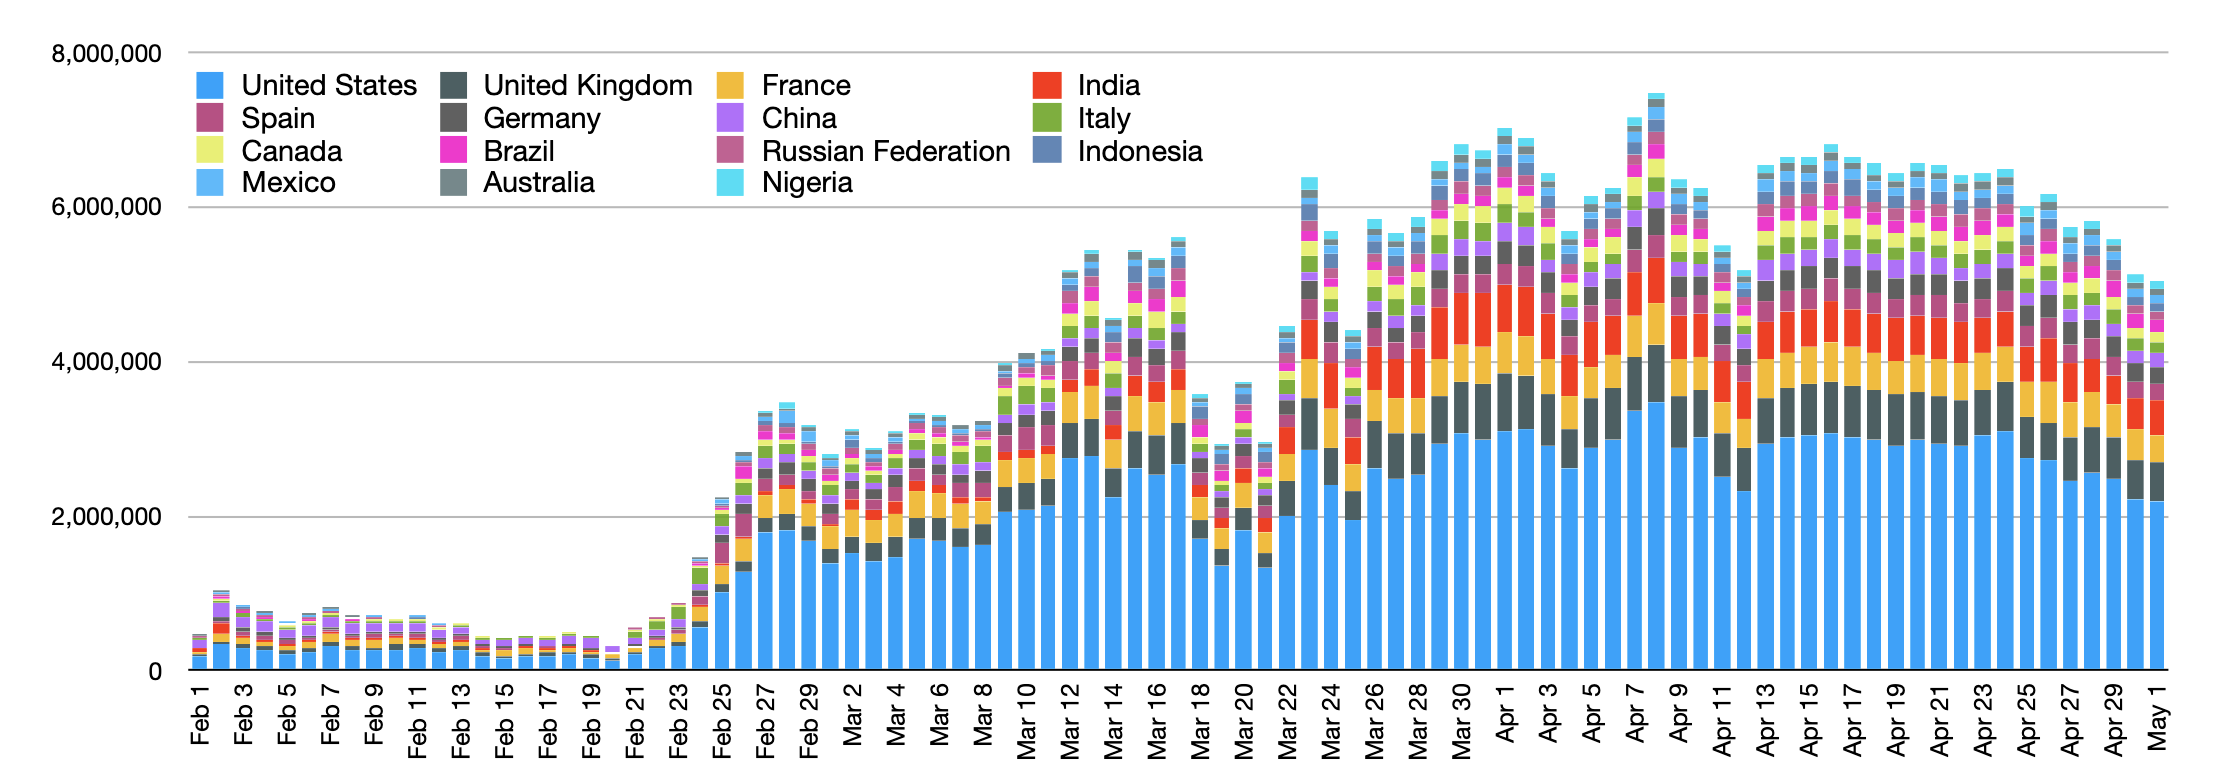
\includegraphics[width=0.8\textwidth]{figs/GeoCov-countrydistribution.png}    
    \centering
    \caption{Daily distribution by country of GeoCoV19 tweets, Feb 1st to May 1st, 2020 \parencite{qaziGeoCoV19DatasetHundreds2020a}}
\end{figure}
%give exact figure instead of 150k here
%https://www.kaggle.com/andradaolteanu/covid-19-sentiment-analysis-social-networks very cool and could be useful!
Note that the volume of tweets captured in the dataset increase very substantially over February and early March, levelling off in mid-March. This gives rise to a potential selection problem, that risk-seeking individuals do not tweet about COVID in February and bias the dataset. This concern is addressed in the main specification, which is discussed in section \ref{methods}.

Of the final dataset, around 150,000 have exact geolocation embedded in the tweet. This is due to the fact that geo-tagging is an explicit option that needs to be set for each tweet, involving activating location data on the mobile app. Another option for geo-tagging is to select a place from a search box; yielding a `place' in the metadata. Both of these types of metadata involve accurate locations, but make up a small proportion of the total geolocated tweets. A third method of geolocating tweets is used to identify most of the locations: when activating a Twitter account the user is strongly encouraged to set their location in their profile. Although it is a free field (generated Place suggestions are included, but are optional), most users set this to their current location; this metadata is included with every tweet. The maintainers of the dataset then employ a toponym extraction approach to elicit the location of the location field. The text of the user location field is first cleaned of non-text characters and symbols. Candidates are then created from the remaining unigrams (single words) and bigrams (pairs of adjacent words), ensuring that two-word place names like `Los Angeles' are included. Groups of three or more words are not considered. Each remaining candidate is filtered against a list of stopwords (see section \ref{textan}), and against the `World Cities Database'\footnote{Available at \texttt{https://www.kaggle.com/max-mind/world-cities-database?select=worldcitiespop.csv}}, an index of 3.1 million worldwide place names, covering 141,989 locations in the US. The remaining candidates are sent as one query to Nominatim, the OpenStreetMap search engine, yielding a best-attempt geolocation: the procedure works best when state and place name is given. Cross-checking the procedure with GPS-geolocated tweets, the dataset shows good coverage and accuracy across US counties, and so makes a panel approach viable. The maintainers of the dataset also presented locations derived from the text of the tweet itself using the same procedure, but we filter these tweets out of the final dataset due to low accuracy. A drawback to this gazeteer approach is that, since users can set their profile location freely, users from other countries or states could masquerade as Americans in particular locations, or the classification process could mis-classify a foreign (particularly English) place as a US location due to sharing a name -- for example, York County, Maine. In order to account for this we remove counties from consideration that have a share of total tweets significantly higher than their population share of the US: Earth, Texas, is the most prominent example of this. Other than misclassification, deliberate setting of the profile location to a US location is possible. This may be a concern for large, well-known cities like Los Angeles and New York, but it is less likely that a given user will set their location to a less well-known American county. Finally, users may move county and not change their location.
\begin{figure}[h!]
    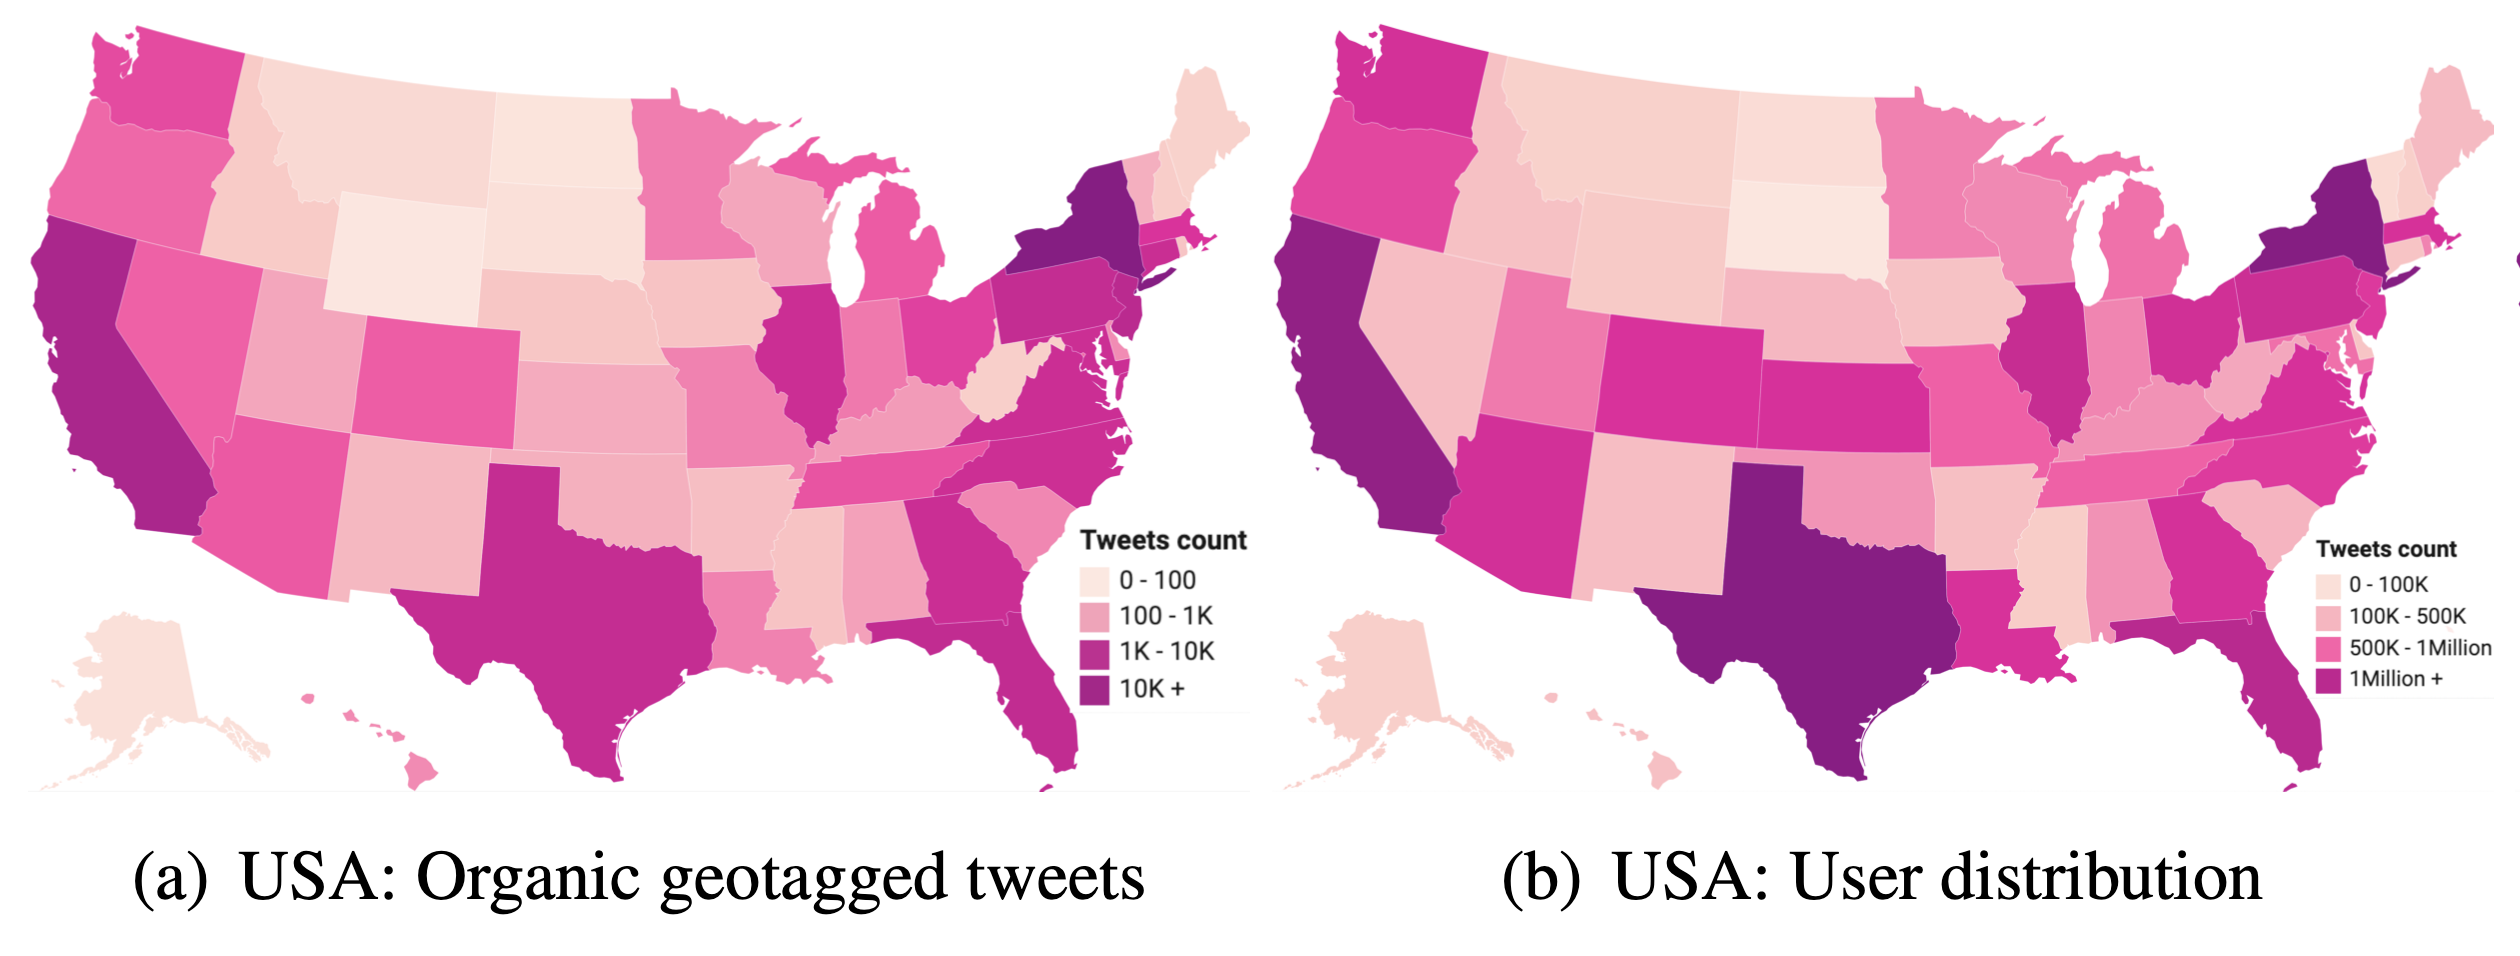
\includegraphics[width=0.8\textwidth]{figs/GeoCov-USdist.png}    
    \centering
    \caption{Geographic distribution of GeoCoV19 tweets and users \parencite{qaziGeoCoV19DatasetHundreds2020a}}
\end{figure}

Twitter's terms of service restrict the large-scale sharing of Tweet datasets; hence public-facing tweet datasets can only be made available `dehydrated', with only the universal identifiers (a long number that maps to the tweet in Twitter's database) given, instead of the tweet text and assorted metadata. In order to use the dataset to analyse tweet content, researchers wishing to use the dataset must apply and be accepted for a Developer account. This gives access to a password called an API key, which is used to query the Twitter API with the identifiers to `rehydrate' and gain access to the full tweet text and metadata. Since the tweets are delivered from the servers at download time, this procedure entails that a proportion of Tweets -- those identified as containing misinformation or those sent by users whose accounts have since been suspended or deleted -- will be unavailable on request from the service when the dataset is `rehydrated'. This presents a selection problem for topics like misinformation, where Twitter enacts a stringent and continuous policy. A prominent concern for my data might be the suspension of Donald Trump's prolific Twitter account; his tweets were a touchstone for right-wing US online conversations. This does not present an issue to my data, however, because tweets interacting with tweets from a deleted account are still available from the API. The deletion rate ultimately encountered during the rehydration process was around 20\%, reflecting the normal removal of machine-generated content.

GeoCoV19 was made available as a dehydrated dataset, containing the tweet identifiers and the inferrred geolocation information. The tweets were rehydrated in December 2020 using Hydrator, an open-source tool made available for academic research by the digital archive organisation Documenting the Now \parencite{summersHydrator2020}. Each tweet is delivered in the Javascript Object Notation (JSON) format: this is a common file standard used to deliver arbitrarily nested data. Each entry contains a `tree', which corresponds to a key-value pair. Each value can itself contain a list of named objects; so, unlike a CSV file, the data is not a `flat' table. An example from the Developer documentation is reproduced below: note the nesting and the metadata delivered with the tweet text. The final dataset contained 63,654,120 tweets and measured approximately 207 GB.

\begin{singlespace}
\begin{lstlisting}[language=json,numbers=none,caption=Example Tweet object JSON file \parencite{twitterinc.DataDictionaryStandard2021}]
{
  "created_at": "Thu Apr 06 15:24:15 +0000 2017",
  "id_str": "850006245121695744",
  "text": "1\/ Today we\u2019re sharing our vision for the future of the Twitter API platform!\nhttps:\/\/t.co\/XweGngmxlP",
  "user": {
    "id": 2244994945,
    "name": "Twitter Dev",
    "screen_name": "TwitterDev",
    "location": "Internet",
    "url": "https:\/\/dev.twitter.com\/",
    "description": "Your official source for Twitter Platform news, updates & events. Need technical help? Visit https:\/\/twittercommunity.com\/ \u2328\ufe0f #TapIntoTwitter"
  },
  "place": {   
  },
  "entities": {
    "hashtags": [      
    ],
    "urls": [
      {
        "url": "https:\/\/t.co\/XweGngmxlP",
        "unwound": {
          "url": "https:\/\/cards.twitter.com\/cards\/18ce53wgo4h\/3xo1c",
          "title": "Building the Future of the Twitter API Platform"
        }
      }
    ],
    "user_mentions": [     
    ]
  }
}
\end{lstlisting}
\end{singlespace}
After the dataset downloaded, a Python script was used to parse and un-nest the JSON files, select the relevant variables, and write them to a CSV file. This file was then joined by matching the UIDs in the CSV with the geolocation dataset in GeoCoV19, yielding a large CSV-format dataset containing the tweet text and metadata from Twitter, and inferred geolocation information from GeoCoV19.

Next, two data cleaning steps were performed. First, it was necessary to drop accounts containing machine-generated content. On Twitter, these are `spambots': accounts that tweet tens of thousands of times per day. The text generated by these accounts does not accurately reflect the local area sentiment, and so must be dropped. We do this by filtering the tweet dataset by user ID, and dropping all tweets by accounts which have posted more than 5,000 tweets over the three-month period. This trims the outlier accounts while keeping the large proportion of the dataset.


Language processing was then performed on the tweet texts, as is detailed in section \ref{approach}. 

\subsection{SafeGraph: Geolocated smartphone data for measuring social distancing}
A second central dataset is provided by SafeGraph, a company which usually collects data on commercial footfall, but made their dataset available for academic research in light of the pandemic. The social distancing dataset was downloaded in January 2020 using the provided API key. The data was parsed and loaded into R using the SafeGraphR package \parencite{huntington-kleinSafeGraphR2020}. The SafeGraph dataset consists of over 45 million anonymised smartphone GPS pings located to an accuracy of a ~150m square location \parencite{safegraphinc.SocialDistancingMetrics2020}. Since the data was collected in 2019 and 2020, year-on-year change can also be presented. The data is presented at district level, but for the purposes of the analysis I aggregated this to a county-level daily metric. For each device on each day, the most common night-time location is determined from the previous 6 weeks. This home location is used to determine the number of devices in a county which leave their home, the length and time of day they leave and return, the district they travel to, and the points of interest they visit. Although this is a sensible method of determining a device's `home', it may be a source of measurement error if an individual works a night shift, does not bring their smartphone with them when they leave the house, or sleeps regularly at a partner's house \parencite{chiouSocialDistancingInternet2020}. However, I believe that the long lead time of 6 weeks' determination, the large sample size, and the rarity of this occurence mitigate the size of the potential measurement error. There is also a chance for selection bias: the data does not represent those Americans who do not own a GPS-enabled smartphone, and does not represent those who refuse to allow GPS tracking on their smartphones. We assume, with evidence, that these omitted populations are mean-zero with respect to social distancing mobility behaviour: 81\% of US adults own a smartphone and 96\% own a cellphone \parencite{pewresearchcenterDemographicsMobileDevice2019}, and \parencite{atheyDigitalPrivacyParadox2017} indicates that the decision to share personal information has a large random element \parencite{chiouSocialDistancingInternet2020}. SafeGraph also address the issue of sampling bias\footnote{\tt{https://colab.research.google.com/drive/1u15afRytJMsizySFqA2EPlXSh3KTmNTQ\#sandboxMode=true}} by comparing, for each census block, the observed proportion of all devices to that census block's proportion of total US population\footnote{That is, if New York County has 3.14\% of the US population, they would expect to find 3.14\% of their total observed devices in New York County}. They assess this sampling bias at the county and demographic level and do not find a significant in observed proportion to that indicated by the census data. From this rich data, I derive two primary variables: the median minutes spent at home during 8am-6pm and the proportion of measured devices that stayed at home all day.  It should be noted that the differential anonymisation means that the exact sum of devices is inaccurate; although there is a possibility to bias the proportions I calculate, this only arises in areas which are sparsely populated. These areas usually do not yield enough geo-located tweets to be included in the final analysis, so the problem is largely circumvented.

\subsection{Other datasets}
\subsubsection{Oxford COVID-19 Government Response Index}
An ongoing feature of the US response to COVID-19 is the differential policies enacted in each state. These policies had varying effects on the extent of social distancing practised in the state and sub-state areas. In order to account for this variation, it is necessary to report the nature and strength of the policy in place in each county at each time point. \textcite{petherickVariationGovernmentResponses2020} provide the \textit{de facto} standard index for tracking government responses. This dataset, originating from the Blavatnik School of Government at Oxford University, reports 19 indicators of government response in containment/control, economic support, and health categories. The containment/control variables are of most interest; these include indicators for school/workplace closures, public transport closures, stay at home requirements, internal/international movement restrictions, restrictions on gathering size, and public event cancellation. These are coded on an ordinal scale (usually 0 to 2, but sometimes 0 to 4), measuring the severity or intensity of the policy. These indicator variables are then aggregated into a `policy stringency' index, a numeric measure of the general severity of restrictions on movement in a governmental area. This index is created by taking the ordinal values of each indicator, rescaling each by the maximum value of the scale, to create a score between 0 and 100. Although this approach inevitably masks substantial subtleties in the context of each policy, they crucially provide a comparable index. The dataset is available at the state level for the US, meaning that it does not cover county-level differences in policy. However, this does not present a problem for the analysis; practically all non-federal COVID containment policies were enacted by blanket state-level orders.

\subsubsection{American Community Survey and Census}
Demographics also have a significant bearing on social distancing behaviour; an area with more elderly people will display less movement than a younger district, due both to baseline movement patterns and differing shielding behaviours during the pandemic. In the main specifcation, we account for this with county fixed effects; but this data is also useful for exploring patterns of sentiment and social distancing among broader demographics. Therefore, I include data from the American Community Survey (ACS) and the 2011 US Census. This includes variables like population density, income, and age distribution. I match the Public Use Microdata Sample of the ACS to the county level, the smallest level available. 

\subsubsection{COVID Case and Death Counts}
COVID-19 case and death counts are provided by the Johns Hopkins University dashboard \textcite{dongInteractiveWebbasedDashboard2020}; we report cases and death counts both cumulatively and daily. In the main econometric specification, deaths are used over reported cases; it is widely accepted that there was a substantial amount of measurement error in the early pandemic, with under-reporting due to low testing and variation in testing capacity over times and regions. Deaths are more accurately and consistently reported, although some measurement error may remain, particularly in February, where some individuals may have died in hospital without being tested for COVID-19. COVID deaths which occur outside of hospital in the early pandemic are also unlikely to have been counted; however, both of these populations are likely to be very small. 




\subsection{Text analyses of Twitter data}\label{approach}
\subsubsection{NRC Emotion Lexicon}\label{nrc}
Sentiment analysis is the task of inferring the author's opinion of a subject from the text they write about that subject. Due to major commercial incentives for accurate sentiment inference from internet companies, this area has seen major advancement over the last 15 years. The NRC Emotion Lexicon is a widely-used tool in this field\footnote{For example, \textcite{mohammadCrowdsourcingWordEmotion2013} -- the paper describing the NRC lexicon -- has been cited over 1,300 times.}; the project aims to answer questions like ``Is the author happy with, angry at, or fearful of the target?'' \parencite{mohammadCrowdsourcingWordEmotion2013}. The lexicon uses the notion that the emotions expressed in a text are a function of the choices of words: that is, words like `gloomy' indicate sadness in a text, `delightful' indicates joy, and so on. The lexicon is composed of a term and the emotion mapped to the term; each term can be mapped to multiple emotions, or none at all. There are eight basic emotions that each word is mapped to: anger, anticipation, disgust, fear, joy, sadness, surprise, and trust; these correspond to \textcite{plutchikGeneralPsychoevolutionaryTheory1980}'s widely-used taxonomy of emotions. The final lexicon contains 14,182 terms annotated with their corresponding emotions. This is large, covering a very wide portion of common English vocabulary. It is also very simple, as it is a binary, one-to-many mapping from term to emotions. This entails that the lexicon takes no account of \textit{intensity} of emotion. It also deals with ambiguous words -- such as the vernacular usage of `sick', which connotes a positive emotion -- in a simple way, by assigning every connected emotion to the term. It is therefore possible that a term could connote every one of the eight emotions. Finally, the lexicon only considers unigrams, which means phrases and multi-word contexts are omitted, and negation is not considered.
\begin{singlespace}
  \begin{table}[!htb]\centering \caption{Sample from NRC Emotion Lexicon \parencite{mohammadCrowdsourcingWordEmotion2013}}
    \begin{tabular}{@{}lcccccccc@{}}
    \toprule
    term        & anger & anticipation & disgust & fear & joy & sadness & surprise & trust \\ \midrule
    aback       & 0     & 0            & 0       & 0    & 0   & 0       & 0        & 0     \\
    abacus      & 0     & 0            & 0       & 0    & 0   & 0       & 0        & 1     \\
    abandon     & 0     & 0            & 0       & 1    & 0   & 1       & 0        & 0     \\
    abandoned   & 1     & 0            & 0       & 1    & 0   & 1       & 0        & 0     \\
    abandonment & 1     & 0            & 0       & 1    & 0   & 1       & 1        & 0     \\ \bottomrule
    \end{tabular}
    \end{table}
\end{singlespace}

Following the download from the Twitter API, the text content and UID of each tweet was separated from the metadata. This uncleaned dataset contains 34.7 million tweets, totalling 7 GB of data. This dataset consists of both tweets and retweets, a function where a user `forwards' somebody else's tweet to their own followers. In order to isolate the possible effect of retweeting another person's opinion, which in some cases may differ from one's own, I filter the full dataset for only original tweets; this `original-only' dataset contains around 6.4 million tweets. NRC sentiment analysis was performed on the full and original-only datasets; due to computational constraints the VADER analysis was performed solely on the original-only dataset. The NRC sentiment analysis uses the same code for both datasets and the pre-processing steps are identical regardless of dataset or analysis technique.

The first cleaning step is to remove links and username mentions from the text, and remove any tweets which are blank. Stop-word removal was not necessary, since the lexicon only matches sentiment-laden terms. Next, the \texttt{sentimentR} package \parencite{rinkerSentimentr2018} is used to split the text into sentences, as we compute the sentiment at the sentence level. Next, the text is split into its constituent tokens using the \texttt{tidytext} package \parencite{silgeTextMiningTidy2017}. The resulting document term matrix is then matched against the NRC lexicon and aggregated at the sentence level; we therefore obtain a binary factor variable for whether words connoting the different emotions appear in each sentence. The `fear' emotion is the variable of interest; the fear factor variable is aggregated back up to the tweet level\footnote{This sentence-level analysis is an artifact of the R packages used to conduct the text-cleaning process; there is no change by aggregating back up to the tweet level after the sentiment analysis is done.}, giving a binary factor for whether words associated with fear appear in the tweet text.  Tf-idf scaling was not performed.

For both sentiment estimation measures, the sentiment scores for the tweets were aggregated to the county level. The NRC score was aggregated by calculating the proportion of tweets in a county on a given day that contained fearful language. If we assume that each tweet is an independent `draw' from the local population, this proportion follows a  binomial distribution, as the variable represents the number of successes -- tweets containing fearful language -- on a sequence of independent Bernoulli trials (tweets in a location on a particular day). We know from the Central Limit Theorem that a binomial distribution approximates a normal distribution with repeated trials; however, for this to be the case, the number of trials on a given day has to be sufficiently large. This means that on days  where the number of observed tweets is low, the proportion of fearful tweets in the observed sample will not be an accurate estimator for the population value. Take the extreme example: in a county where there is one observed tweet on a given day, the value of the proportion can only be 0 or 1. With repeated sampling, the proportion will converge to the population proportion, but this N has to be sufficiently large. This effect gives rise to a shape of the histogram of county-day proportions for the whole dataset, where we observe an increase in density at 0 and 1. The central limit theorem does not specify a lower bound sample size to alleviate this issue, but 30 is a common approximation. Hence, in order to rectify the inaccurate estimators for small-\(n\) county/days, we exclude county/days where the number of tweets is below 30. In doing so, we discard around 8.1\% of the data. This procedure, however, means that the panel is unbalanced based on tweet count; this possible selection effect is discussed in section \ref{robust}. The histogram and quantile plots for the fear proportion variable are figures \ref{n30_hist} and \ref{n30_qplot} in appendix \ref{add-figs}: we observe that, although the tails are heavy, the distribution is a fair approximation to normal.

\begin{figure}[h!]
  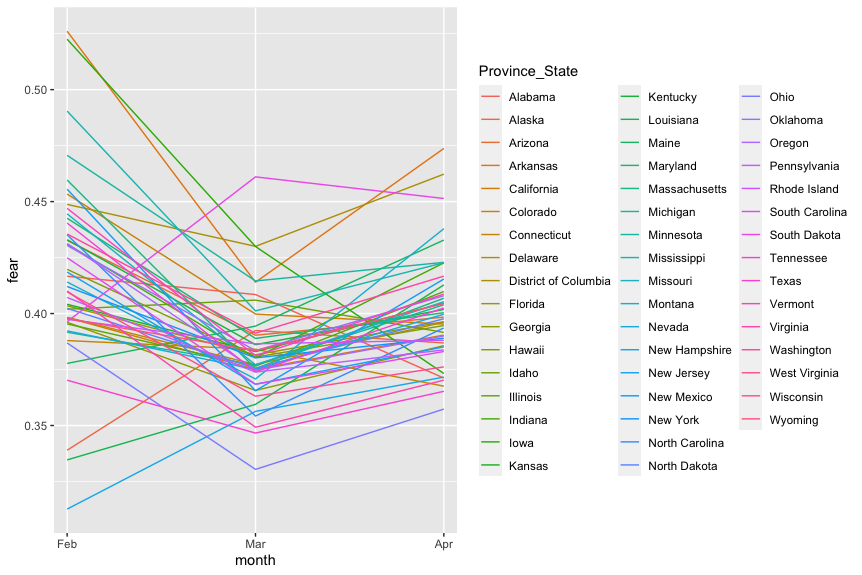
\includegraphics[width=0.8\textwidth]{figs/sent_time.png}    
  \centering
  \caption{Proportion of fearful tweets, averaged at state/month level.}
  \label{sent_time}
\end{figure}


As we observe in figure \ref{sent_time}, the variation in sentiment is greater earlier in the pandemic in February than later on in March and April.  The figure indicates that expressed fear \textit{decreased} on the aggregate during March, followed by an increase in April. This may be dubious, as we might expect fearful tweets to increase during the critical March period: however, this graph does not take covariates and county-level effects into account. The variation in sentiment observed across states in February is evidence counting against the existence of an early-stage selection effect, where only those fearful of the virus tweet about it early on: if this were the case, then we would expect that all states' fear levels should be high in February,given that the virus had not substantially spread anywhere in the US at that point.

\subsubsection{VADER Rule-Based Sentiment Approach}\label{vader}
A key identifying assumption of the research design is that the sentiment procedure accurately reflects the latent variable of `local sentiment'. Since sentiment is fundamentally unobserved this assumption is difficult to robustly test, but a strong signal for accuracy is if the results can be replicated using different ways of measuring sentiment. Additionally, the NRC method has certain drawbacks: although it has the advantage of yielding emotion scores, allowing the analysis to pick out the `fear' dimension of each tweet text, it lacks sophistication. In particular, in addition to the problems with ambiguity, omission of multi-grams, and lack of negation mentioned above, the lexicon is not \textit{domain-specific}. On Twitter, as with all online platforms, emojis (for example) take on a significant role for communication; additionally, the platform has its own manner of communication which is different to other forms of writing. This means that certain emotions may be mis-allocated, or -- in the case of emojis -- omitted altogether. This motivates the use of an alternative text analysis tool, which is designed for sentiment analysis on the Twitter platform. The `Valence Aware Dictionary for sEntiment Reasoning' (VADER, \textcite{huttoVaderParsimoniousRulebased2014}) is a popular tool for Twitter-based sentiment analysis, and both addresses our sophistication concerns and allows us to test the validity of the identifying assumption.

VADER is considered to be the gold-standard for social media sentiment lexicons, and performs equally well as human raters at matching sentiments. Instead of emotions, however, VADER reports sentiment as a \textit{polarity} score. In the broadest sense, polarity is a binary measure of the disposition of the author towards the topic of the text, and is either positive, neutral, or negative. The polarity score can also reflect the intensity of the disposition; for example, compare `exceptional' to `okay'. VADER takes into account the intensity of valence, and so reports its polarity index on a continuous scale. When using VADER, the polarity can be reported at the text level, but this text polarity score is always an aggregate function of the term polarities. This aggregate function might include, for example, term frequency / inverse document frequency (tf-idf) weighting (as discussed in section \ref{preprocess}), perhaps in addition to some transformation which takes into account the context of each term.

VADER is also able to identify the contextual meaning of terms by using a pre-trained sentiment classifier, and additionally incorporates five rules extracting meaning from word order and grammar. These are punctuation, capitalisation, degree modifiers (e.g. `extremely', `marginally'), `but' as a signal of polarity shift, and a sophisticated negation detector. This final rule examines the trigram before a sentiment-laden term (above a certain absolute value) and determines if it has been negated; this rule achieves 90\% accuracy. Crucially, all the lexical features VADER includes are calibrated and verified to identify sentiment on the Twitter platform. In general, VADER performs as well or better than cutting-edge, compute-heavy sentiment extractors on Twitter data. 

The R package \texttt{vader} \parencite{roehrickVaderValenceAware2020} is used to perform the sentiment analysis. Due to the extensive memory requirements of the analysis process, the uncleaned tweets dataset was split into 64 files of 100,000 tweets each and the code run on a virtual machine on the Google Cloud Compute platform. The same cleaning pre-processing was performed: removing links, usernames, and hashtags. The sentiment analysis calculates the polarity of each word in the sentence on a continuous scale, and reports the  individual word scores, the compound polarity score (normalised to a continuous \([-1,1]\) scale from the sum of the individual sentiment scores), and the adjusted proportion of the text that is positive (and likewise for negative and neutral. Note that the adjusted proportion of the score accounts for both text length and text intensity, reflecting a higher score for higher intensity and similar results regardless of length. An example of the output from the VADER program is in appendix \ref{add-figs}.

The aggregation procedure for the VADER package is broadly similar to the NRC lexicon: the mean for the individual tweet sentiment is calculated at the county/day level, with counts below thirty dropped from the dataset. Visually, the compound measure is symmetrical around 0, with other modes at around \(\pm 0.5\). The distribution of the county/day mean sentiment is skew, centered around \(0.1\)\footnote{See figures \ref{comp_hist}, \ref{meancomp_hist} in Appendix \ref{add-figs}.}.

\subsection{Descriptive statistics}\label{descrip}
\begin{singlespace}
    \begin{table}[!htb]
    \centering  
  \caption{Descriptive statistics, all US counties, Feb 1 - May 1 2020}
  \begin{tabular}{lcccc}
    \toprule
     & Mean & Std Dev & Min & Max\\
    \midrule
    Deaths, cumulative & 58.6 & 211.6 & 0 & 4710\\
    Cases, cumulative & 1374.9 & 3701.8 & 0 & 53032\\
    \addlinespace
    \% 65+ & 13.5 & 3.6 & 6.5 & 51.6\\
    Persons per HH & 2.5 & 0.23 & 2 & 4\\
    HH Income (000s) & 55.77 & 12.73 & 20.97 & 122.24\\
    \% Below poverty level & 16.3 & 4.4 & 3.6 & 39.2\\
    Population per sq. mile & 2593 & 5560 & 0.2 & 69468\\
    \addlinespace
    National Stringency Index & 60.89 & 22.78 & 0 & 72.69\\
    State Stringency Index & 56.45 & 25.68 & 0 & 87.96\\
    \addlinespace
    Tweets per week & 10546 & 14560 & 41 & 55263\\
    \addlinespace
    Device Count & 52913 & 59662 & 72 & 344342\\
    \% Devices at home & 37.46 & 8.96 & 11.50 & 63.11\\
    \bottomrule
    \end{tabular}
  \floatfoot{All variables reported at county level. Stringency indices bounded between 0 and 100. Household income as measured in 2013 US dollars, unadjusted.}
  \end{table}
\end{singlespace}
The primary dependent variable is `\% devices at home'; that is, the proportion of devices on a given county-day which stay completely at home. It has a mean of 37\%; as expected, it is strongly correlated with time. \textit{Some comments on the distribution and variation here}. Tweets per week and device count have a very large range, since these track with county population (which is very variable, unlike voting districts: Los Angeles county has 10 million residents, for example). However both variables show little per capita variation, pointing to consistent sampling across the whole of the US: in this way, sampling bias on these variables is unlikely. Deaths and cases are path-dependent, as New York City and Seattle acquired serious outbreaks earlier than other areas. Data is reported for all 3,142 counties over the 90 days between February 1 and May 1 2020.

\section{Methods}\label{methods}
\begin{figure}[!htb]
  \centering
  \caption{Overview of data collection, processing, and estimation.}\label{process}
  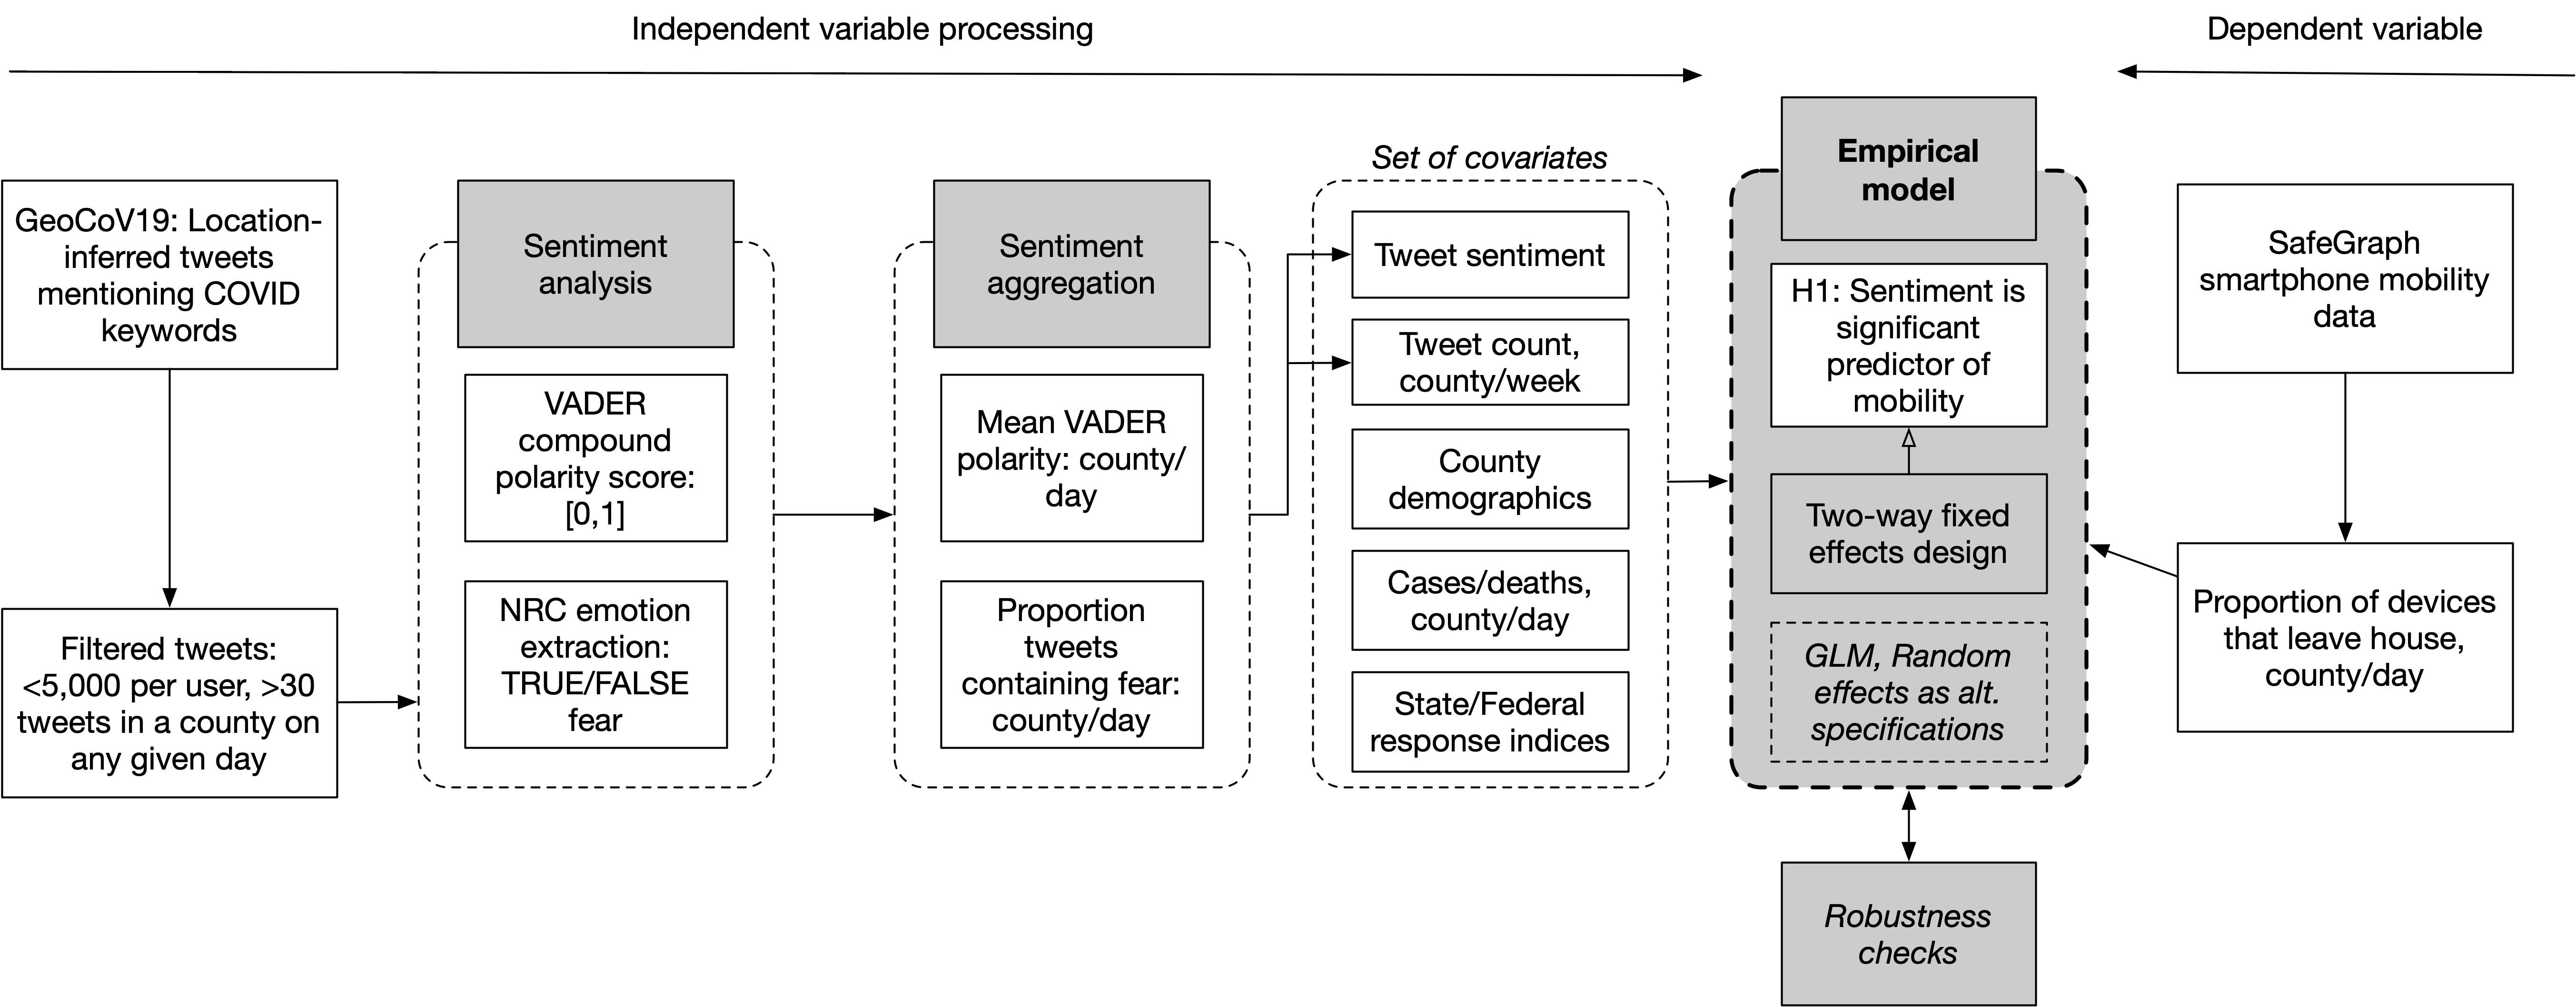
\includegraphics[width=0.9\textwidth]{figs/processing.png}
\end{figure}
\subsection{Central Argument and Empirical Specficiation}
The primary aim of this dissertation is to investigate whether there is a link between individual risk preferences and social distancing. Previous research has established several important factors in predicting mobility in response to health risks: in addition to policy orders, demographic variables like individual susceptibility, political affiliation, and the progression of disease, characteristics like risk preference have been identified as key determinants of social distancing. The argument of the dissertation turns on the asssertion that risk preferences vary by region, a notion backed up by the influential Global Preferences Survey \parencite{falkGlobalEvidenceEconomic2018} and applied to the COVID-19 pandemic by \textcite{fanHeterogeneousActionsBeliefs2020}. I assert that this risk preference can, to some extent, be measured by a novel data source: what people say on social media. Using a very large dataset of tweets which mention COVID-19, I argue that those who are risk averse will post more negatively about COVID-19; furthermore, the location of these users indicates a level of risk preference that is shared among those in the local area. This is because complex combinations of local factors -- factors such as the trust in that particular area's local government, the pattern of supply shortages in that area's supermarket, the quality of public transport, and the commuting practises of the area -- all contribute to a shared local perception of pandemic risk. I assert, then, that this shared perception is measured by the local chatter on social media, and I measure it by creating a county-level index of social media sentiment towards COVID-19. We are interested in whether this county index is able significantly to predict the level of social distancing that an area practises.

This dissertation does not aim for a causal identification, but focuses on investigating the extent to which the social distancing and social sentiment are correlated. To that end, I estimate the following specification, where a vector of social distancing metrics in county \(c\) on date \(t\) and week \(w\) is a function of

\begin{equation}
  \label{eq:mainspec}
  SD_{ct} = \beta_1 Sent_{ct} + \beta_2 TweetCount_{ct} + \beta_3 AtHome_{ct} + \beta_4 NatStringency_{t} + \beta_5 Deaths_{ct} + \gamma_c + \delta_w
\end{equation}. The sentiment effect is captured by \(\beta_1\) and \(\beta_2\), policy effects by \(\beta_3\) and \(\beta_4\), and local health risk and disease spread by \(\beta_5\). This primary specification captures the local effects of sentiment, as discussed above; in order to account for the Februrary selection effect discussed in section \ref{geocov}, where far lower COVID tweets observed in Februrary could indicate only those fearful of the virus tweeting about it, we include the number of tweets observed in the county on that week as a covariate. Including this possible confounder in the regression allows for the effect of low observations to be separated from the true effect of tweet sentiment. As such, our primary hypothesis has the first and second coefficients as the effect of interest such that

\begin{align*}
  H_0 : &\: \beta_1 = \beta_2 = 0 \\
  H_1 : &\: \beta_1 \neq \beta_2 \neq 0
\end{align*}, where \(\beta_1\) has the appropriate sign according to its metric, \(\beta_2 > 0\), and the coefficients are jointly and individually significant.


The third, fourth, and fifth coefficients cover time-varying factors like the imposition of policy orders and the spread of the virus. \(\beta_5\) represents not only viral spread, but can act as a proxy for perceived local health risk: this follows \textcite{chernozhukovCausalImpactMasks2021}, in whose model COVID death counts represent the time-varying local and national beliefs on the seriousness of the pandemic. It is important to note that a central identifying assumption in the two-way fixed effects design is that there is no source of time-varying, unobserved heterogeneity: thus it is important to verify that the correct specification is chosen for these time-varying confounders. Finally, \(\gamma_c\) is a vector of county-level fixed effects, capturing all constant demographic variables like percent above 65, income, commuting patterns, etc.; \(\delta_w\) is a vector of week fixed effects, capturing among others the national-level disease spread and health risk perception. All regressions have two-way White heteroscedasticity-robust standard errors, clustered at the county and week level.



\subsubsection{Variables}
We have estimated two measures of tweet sentiment. Both of the measures estimate the sentiment of individual tweets, \(\hat{\mathbf{V}}\), from the raw text \(\mathbf{C}\). For the NRC lexicon, this is a binary measure: `tweet contains fear-related words' is true or false. For each county in each day, a proportion of the tweets contain fear-related words. This proportion is the reported variable. Similarly, the VADER measure is a bounded index over \([-1,1]\), but does not arise directly from count data. The mean of this measure is taken over each county and day, which forms the aggregation procedure. AtHome is an indicator variable for whether the state had imposed a stay-at-home order; and NatStringency reports the the Oxford stringency index, which is normalised to between 0 and 100. Finally, the deaths in each county are included as a time-varying factor; as discussed above, these offer a less biased estimate of the spread of the virus than reported cases, which vary by region and do not include asymptomatic cases. The dependent variables are two mobility measures: the median time spent at home during working hours (expressed as a percentage), and the proportion of measured devices that stay at home all day.

\subsection{Inference with Panel Fixed Effects}
The chosen model is a two-way, time and location fixed effects design. This empirical model is very common with a panel dataset measured at the county level, as the location fixed effect flexibly controls for all unobserved, time-invariant factors in each county. Moreover, the time fixed effect accounts for time-varying factors that are common to all counties -- like the progression of the virus on the world stage, and the level of `shared' sentiment towards COVID across the U.S. 

The fixed effects model is characterised by the linear model  
\begin{equation}
  E[Y_{it} | A_i , X_{it}, t] = \alpha + \lambda_t + A^\prime_i \gamma + X^\prime_{it} \beta + \rho D_{it}
\end{equation}
, where \(Y_{it}\) is the outcome, \(\alpha\) the intercept, \(\lambda_t\) the time effect, \(A^\prime_i \gamma\) unobserved, fixed confounders, \(X^\prime_{it} \beta\) observed time-varying confounders, and \(\rho D_{it}\) the variable of interest \parencite[222]{angristMostlyHarmlessEconometrics2009}. The assumptions are that the effect of \(\rho\) is additive and constant, and that the unobserved fixed effects do not vary with time\footnote{That is, the omission of a time subscript on \(A^\prime_i \gamma\) is accurate.}. In our case, both assumptions are plausible. This directly implies the model 
\begin{align}
  Y_{it} &= \alpha_i + \lambda_t + \rho D_{it} + X^\prime_{it} \beta + \epsilon_{it}, \textrm{, where} \\
  \alpha_i &\equiv \alpha + A_i^\prime \gamma
\end{align}. In this way we estimate the (potentially large number of ) unobserved confounders as the \textit{fixed effect} \(\alpha_i\), which enters into the model as a coefficient on an indicator for each region, and also include a \textit{time effect} \(\lambda_t\). With these effects meted out, we are able to obtain a consistent estimator for the overall, shared effect of our variable of interest, under the assumption that the time-varying confounders are adequately specified. %Maybe comment on measurement error here, too.



\section{Results}%1000 words
\subsection{Main Specification}
The basic message of the main specification can be seen in figure \ref{setsplit} in appendix \ref{add-figs}, which shows that counties with a fear sentiment above the median value have 3 percentage points more devices staying at home. Below is the regression table for the main specification as in equation \ref{eq:mainspec}, which uses the NRC-derived proportion of fearful tweets as the sentiment measure. The two dependent variables are 

\begin{singlespace}
\centering
\begin{table}[!htb]
\caption{Main Specification: NRC Sentiment}
\label{tab:mainspec}
\ra{0.6}
\begin{tabular}{lcccc}
  \tabularnewline\midrule\midrule
  Dependent Variables:&completely\_home\_device\_count&at\_home\_prop&completely\_home\_device\_count&at\_home\_prop\\
  Model:&(1) & (2) & (3) & (4)\\
  \midrule \emph{Variables}&   &   &   &  \\
  meanfear&984.8$^{**}$ & 0.0088$^{*}$ &    &   \\
    &(357.5) & (0.0050) &    &   \\
  at\_home\_orderTRUE&704.2$^{**}$ & 0.0295$^{***}$ & 716.4$^{**}$ & 0.0295$^{***}$\\
    &(267.5) & (0.0039) & (263.7) & (0.0039)\\
  NAT\_StringencyIndex&106.6$^{***}$ & 0.0030$^{***}$ & 106.7$^{***}$ & 0.0031$^{***}$\\
    &(10.68) & (0.0003) & (10.98) & (0.0003)\\
  death&-11.84$^{**}$ & $-6.6\times 10^{-5}$$^{**}$ & -11.64$^{**}$ & $-6.77\times 10^{-5}$$^{**}$\\
    &(4.757) & ($2.34\times 10^{-5}$) & (4.663) & ($2.32\times 10^{-5}$)\\
  confirmed&1.244$^{***}$ & $8.17\times 10^{-6}$$^{***}$ & 1.230$^{***}$ & $8.32\times 10^{-6}$$^{***}$\\
    &(0.4063) & ($2.25\times 10^{-6}$) & (0.4007) & ($2.24\times 10^{-6}$)\\
  meanneg&   &    & 1,011.1 & 0.0606$^{*}$\\
    &   &    & (2,458.5) & (0.0339)\\
  \midrule \emph{Fixed-effects}&   &   &   &  \\
  week & Yes & Yes & Yes & Yes\\
  FIPS & Yes & Yes & Yes & Yes\\
  \midrule \emph{Fit statistics}&  & & & \\
  Observations & 16,474&16,474&16,239&16,239\\
  Log-Likelihood & -156,190.7&31,715.0&-153,815.7&31,229.2\\
  AIC & 313,611.3&-62,199.9&308,861.4&-61,228.4\\
  BIC & 318,352.7&-57,458.6&313,593.9&-56,495.8\\
  RMSE & 3,172.0&0.03529&3,143.4&0.03537\\
  Size of the 'effective' sample & 16,474&16,474&16,239&16,239\\
  F-test & 452.59&160.71&439.90&157.64\\
  F-test (projected) & 542.12&710.57&531.23&703.27\\
  \midrule\midrule\multicolumn{5}{l}{\emph{Two-way (week \& FIPS) standard-errors in parentheses}}\\
  \multicolumn{5}{l}{\emph{Signif. Codes: ***: 0.01, **: 0.05, *: 0.1}}\\
  \end{tabular}
\end{table}

\end{singlespace}


\subsection{Alternative model specifications}\label{alt-specs}
The variable used for the mobility data, and presented as the dependent variable, is the proportion of the measured devices which stay at home all day. Hence, the variable is continuous and bounded between 0 to 1. Although the primary specification is with ordinary least squares, we may wish to address the problem that OLS can identify values beyond \([0,1]\). This quality of the dependent variable may indicate a logit transformation followed by OLS estimation, a generalised linear model with a binomial link function, or a beta regression. 
\subsection{Robustness checks}\label{robust}
As discussed in section \ref{nrc}, a potentially problematic feature of the tweet data is that the number of tweets observed in a county track with the county population. This is a problem because the aggregation procedure for the sentiment index required a minimum of 30 observations for unbiasedness, so all county/days with tweets lower than this number were dropped. This means that the panel we created for the primary specification is unbalanced, with data missing not at random. This may present a selection effect, since population, the variable causing this selection, may be correlated with the dependent variable of mobility. The selection effect can be ignored if we can show that the variable driving the selection is uncorrelated with the dependent variable \parencite[552]{wooldridgeEconometricAnalysisCross2010}. 
\begin{figure}[!htb]
  \centering
  \caption{Scatterplot of county population against daily mobility score.}
  \label{popvsmobil}
  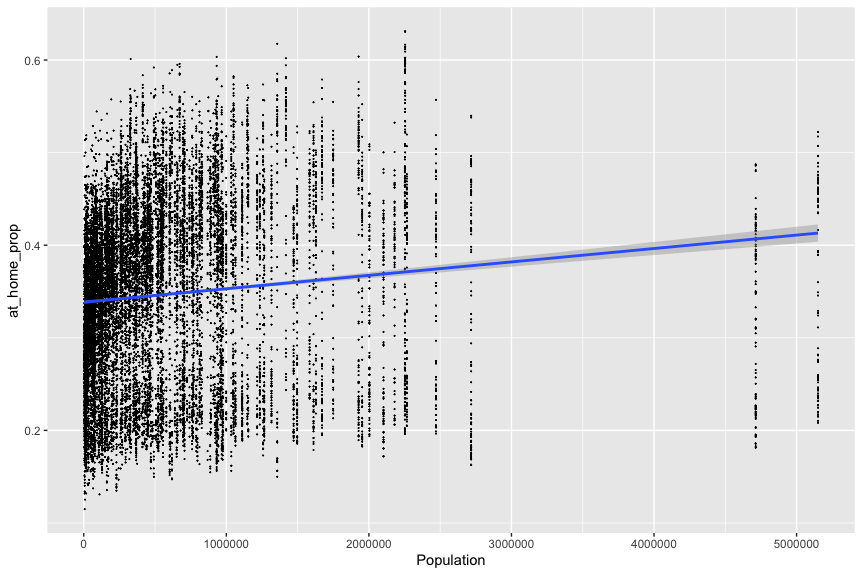
\includegraphics[width=0.6\textwidth]{figs/popvsmobil.png}
  \floatfoot{The vertical lines in the diagram correspond to counties with mobility scores observed at different dates.}
\end{figure}
On visual inspection of figure \ref{popvsmobil}, a positive relationship does exist between the proportion staying at home and the county population (meaning that higher-population counties have \textit{decreased} mobility); however, it appears that this is primarily driven by the two large county outliers. These correspond correspond to the highly dense Los Angeles County and Cooke County, Illinois\footnote{i.e., Chicago}. Discounting these highly dense outlier cities, we can tentatively say that mobility is largely independent of county population. As a consequence, an unbalanced panel could be accomodated. The Heckman correction procedure would be another option for obtaining unbiased parameter estimates \parencite{wooldridgeSelectionCorrectionsPanel1995}, as would weighting the samples by population; and the final option is to avoid aggregating the sentiment scores and run the empirical specification on the individual level. That is, the base unit is an individual tweet rather than the county/day. This yields a much larger panel of the individual observations; the results from runnning this analysis with the main specification are discussed below.


\section{Discussion and conclusion} %1000 words


\printbibliography
%TC:ignore
\newpage

\appendix 
\section{Regression Tables}
\begin{landscape}
  

\begin{table}
\centering
\caption{Retweets MainSpecs}
\begin{tabular}{lcccccc}
  \tabularnewline\midrule\midrule
  Dependent Variables:&home\_count&median\_pct\_time\_home&home\_prop&home\_count&median\_pct\_time\_home&home\_prop\\
  Model:&(1) & (2) & (3) & (4) & (5) & (6)\\
  \midrule \emph{Variables}&   &   &   &   &   &  \\
  meanfear&984.8$^{**}$ & 2,637.5$^{***}$ & 0.0088$^{*}$ &    &    &   \\
    &(357.5) & (795.0) & (0.0050) &    &    &   \\
  at\_home\_orderTRUE&704.2$^{**}$ & 1,027.8$^{**}$ & 0.0295$^{***}$ & 705.7$^{**}$ & 1,027.7$^{**}$ & 0.0294$^{***}$\\
    &(267.5) & (394.6) & (0.0039) & (267.5) & (395.0) & (0.0039)\\
  NAT\_StringencyIndex&106.6$^{***}$ & 157.0$^{***}$ & 0.0030$^{***}$ & 107.1$^{***}$ & 159.7$^{***}$ & 0.0031$^{***}$\\
    &(10.68) & (32.68) & (0.0003) & (10.89) & (32.95) & (0.0003)\\
  death&-11.84$^{**}$ & -19.56$^{**}$ & $-6.61\times 10^{-5}$$^{**}$ & -11.84$^{**}$ & -19.56$^{**}$ & $-6.6\times 10^{-5}$$^{**}$\\
    &(4.757) & (8.729) & ($2.34\times 10^{-5}$) & (4.760) & (8.745) & ($2.34\times 10^{-5}$)\\
  confirmed&1.244$^{***}$ & 2.105$^{**}$ & $8.17\times 10^{-6}$$^{***}$ & 1.243$^{***}$ & 2.104$^{**}$ & $8.17\times 10^{-6}$$^{***}$\\
    &(0.4063) & (0.7757) & ($2.25\times 10^{-6}$) & (0.4067) & (0.7775) & ($2.25\times 10^{-6}$)\\
  meanneg&   &    &    & 909.7 & 6,199.0 & 0.0603\\
    &   &    &    & (2,446.3) & (4,331.9) & (0.0345)\\
  \midrule \emph{Fixed-effects}&   &   &   &   &   &  \\
  week & Yes & Yes & Yes & Yes & Yes & Yes\\
  FIPS & Yes & Yes & Yes & Yes & Yes & Yes\\
  \midrule \emph{Fit statistics}&  & & & & & \\
  Observations & 16,474&16,474&16,474&16,474&16,474&16,474\\
  Log-Likelihood & -156,190.6&-161,812.5&31,715.0&-156,194.2&-161,821.8&31,719.5\\
  BIC & 318,352.5&329,596.4&-57,458.7&318,359.8&329,615.0&-57,467.7\\
  RMSE & 3,171.9&4,462.0&0.03529&3,172.6&4,464.6&0.03528\\
  Size of the 'effective' sample & 16,474&16,474&16,474&16,474&16,474&16,474\\
  F-test & 452.59&1,983.2&160.71&452.38&1,980.9&160.81\\
  F-test (projected) & 542.16&791.18&710.59&540.51&786.71&712.73\\
  \midrule\midrule\multicolumn{7}{l}{\emph{Two-way (week \& FIPS) standard-errors in parentheses}}\\
  \multicolumn{7}{l}{\emph{Signif. Codes: ***: 0.01, **: 0.05, *: 0.1}}\\
  \end{tabular}
\end{table}
\end{landscape}
\section{Additional Figures} \label{add-figs}
\begin{figure}[h!]
  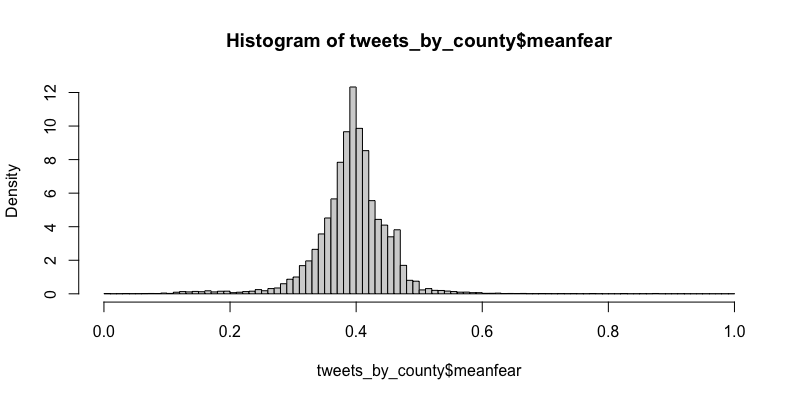
\includegraphics[width=0.8\textwidth]{figs/n30_hist.png}    
  \centering
  \caption{Histogram, proportion of tweets containing fearful language by county/day.}
  \label{n30_hist}
  \floatfoot{Variable presented after trimming county/day buckets with \(n < 30\)}
\end{figure}
\begin{figure}[h!]
  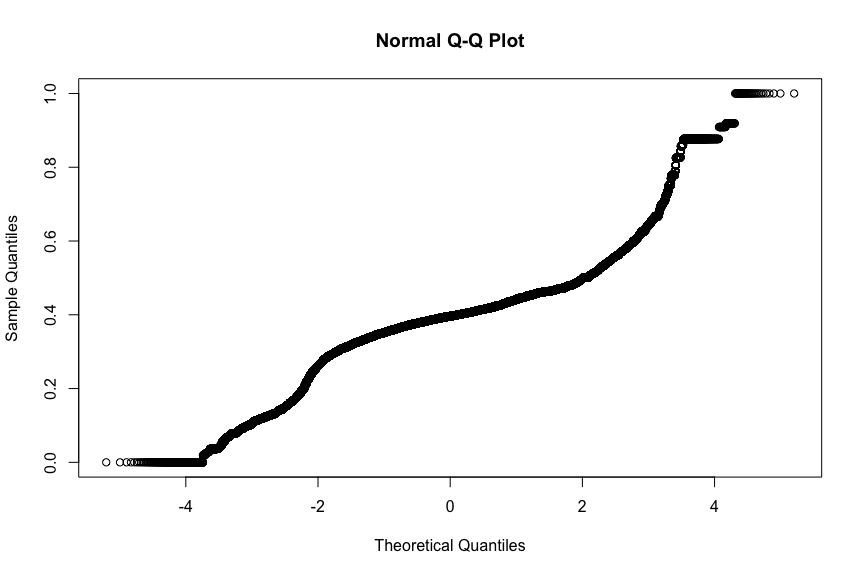
\includegraphics[width=0.8\textwidth]{figs/n30_qplot.png}    
  \centering
  \caption{Normal distribution Quantile-Quantile plot, proportion of tweets containing fearful language by county/day.}
  \label{n30_qplot}
  \floatfoot{Variable presented after trimming county/day buckets with \(n < 30\)}
\end{figure}
\begin{figure}[h!]
  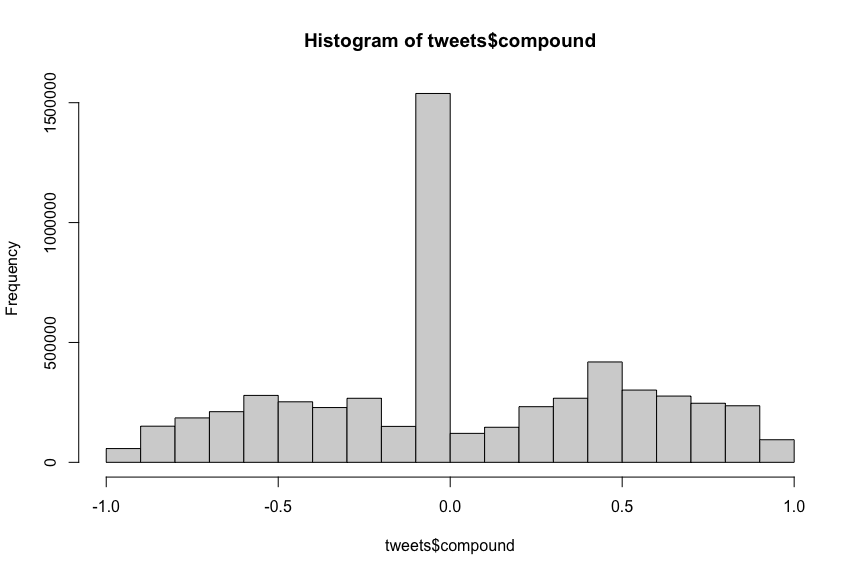
\includegraphics[width=0.8\textwidth]{figs/compound_hist.png}    
  \centering
  \caption{Histogram, individual VADER sentiment scores, compound positive/negative.}
  \label{comp_hist}
  
\end{figure}

\begin{figure}[h!]
  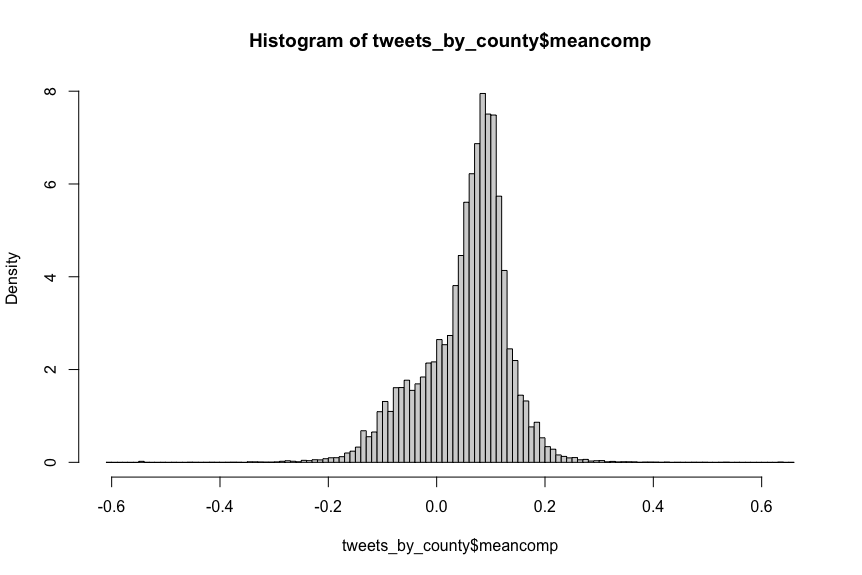
\includegraphics[width=0.8\textwidth]{figs/meancomp_hist.png}    
  \centering
  \caption{Histogram, mean VADER sentiment scores, compound positive/negative.}
  \label{meancomp_hist}
\end{figure}


\begin{figure}[!htb]
  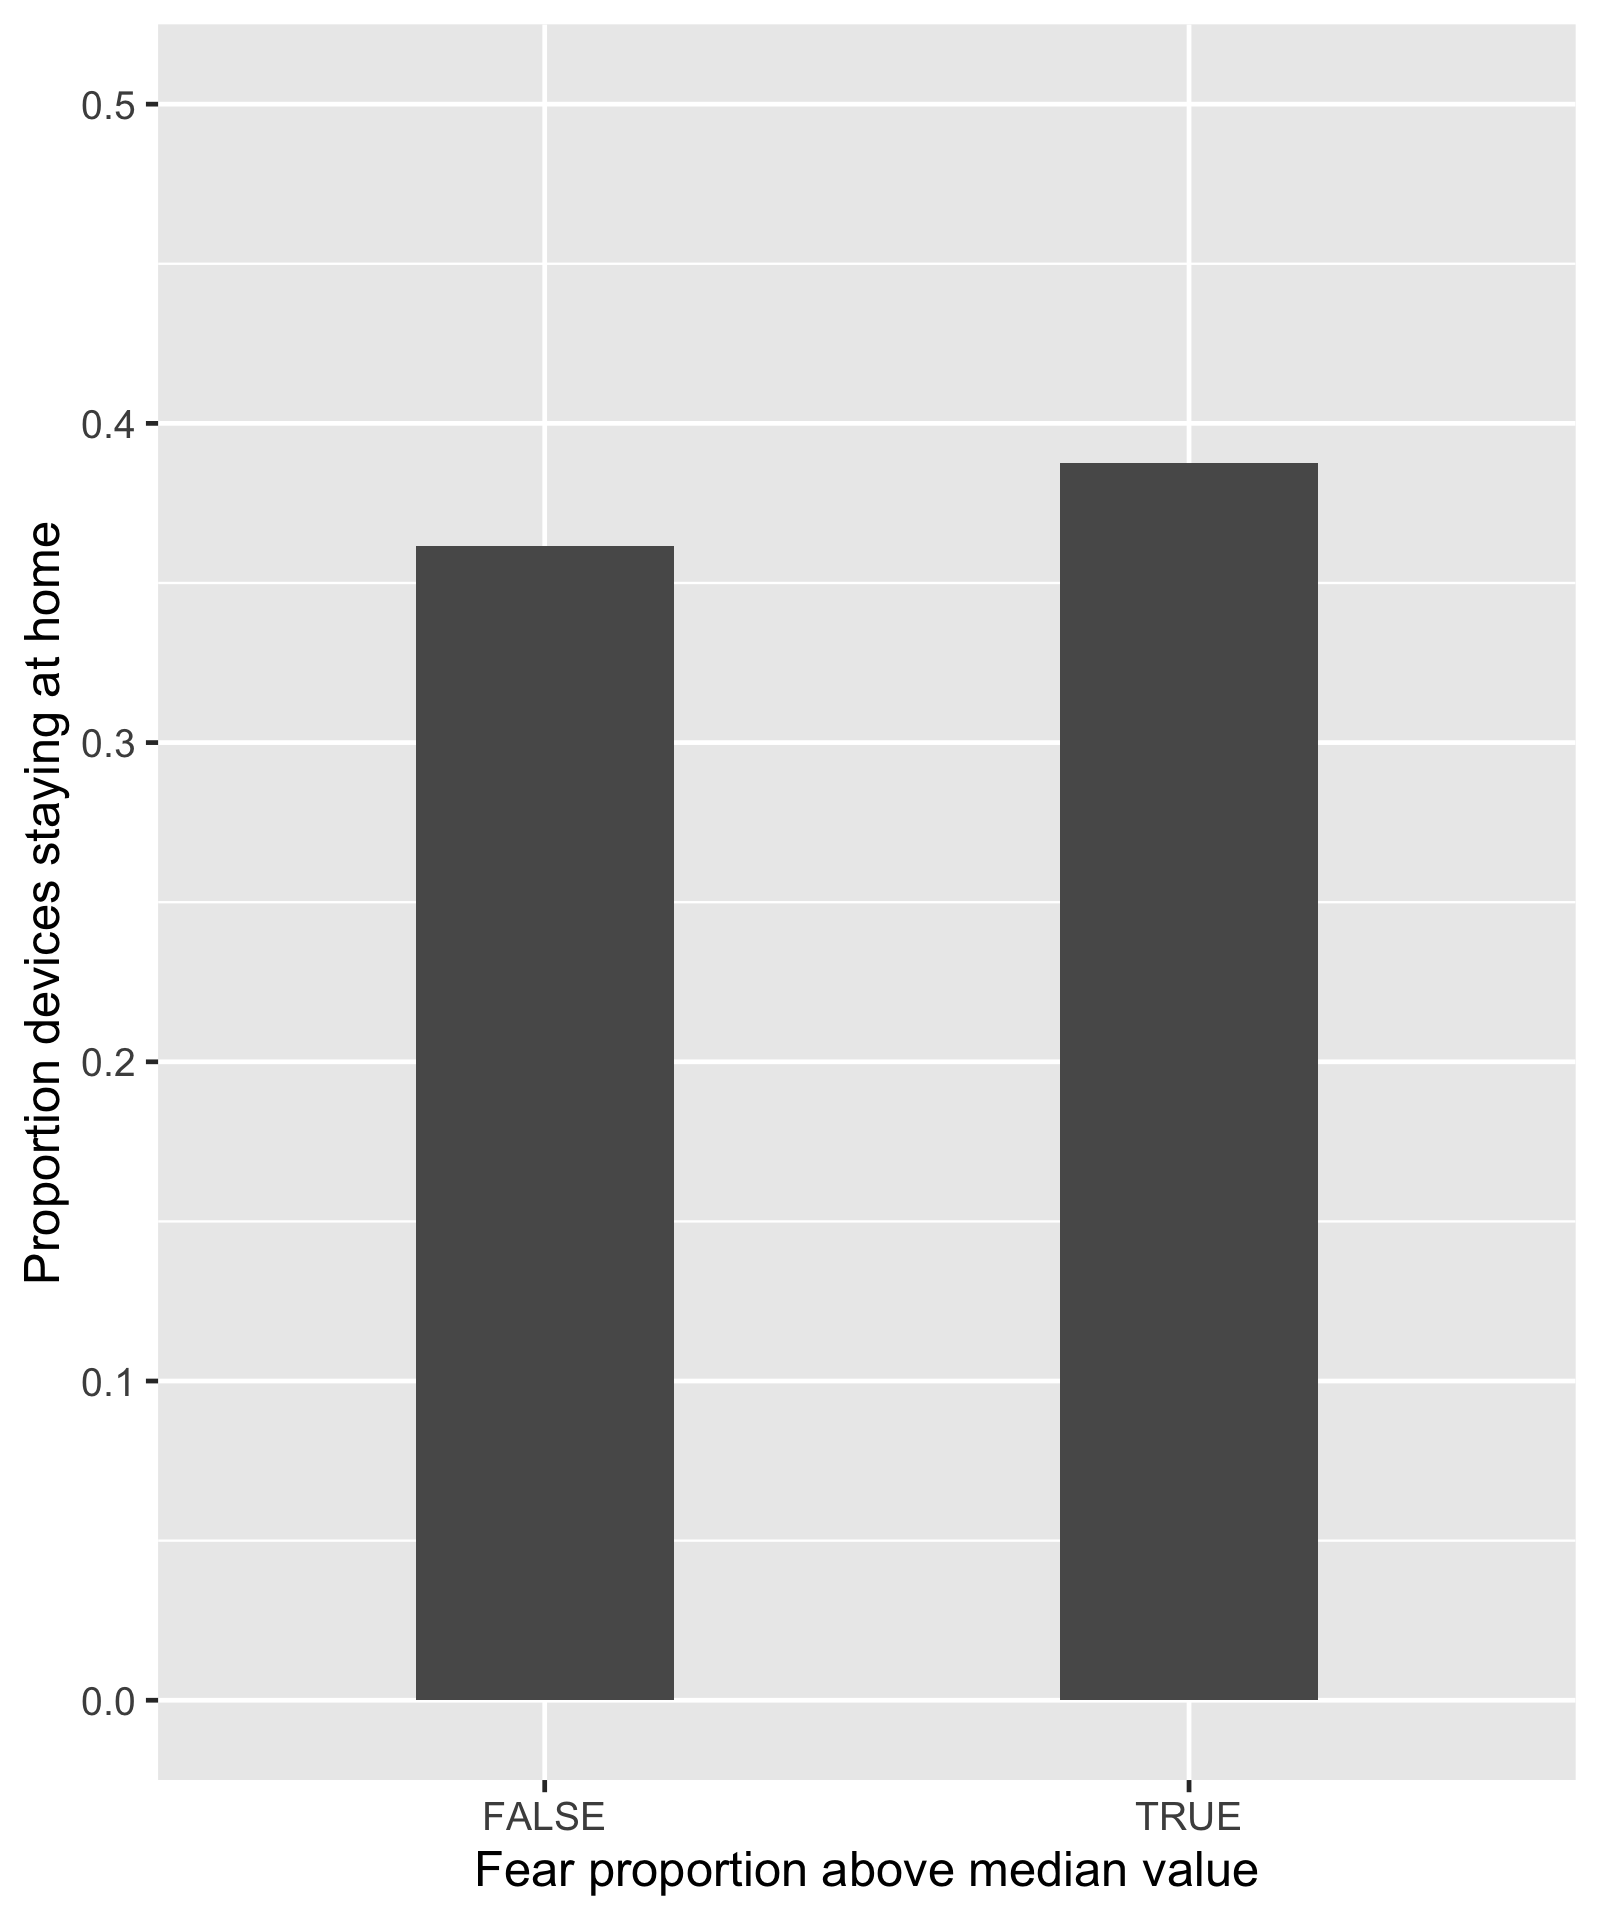
\includegraphics[width=0.5\textwidth]{figs/setsplit.png}    
  \centering
  \caption{Bar chart, comparing mobility in low-fear counties with high-fear counties.}
  \label{setsplit}
  \floatfoot{Low/high fear defined as above or below median proportion of fearful tweets.}
\end{figure}


\begin{landscape}
  \vspace{1.5in}
  \begin{figure}[h!]
    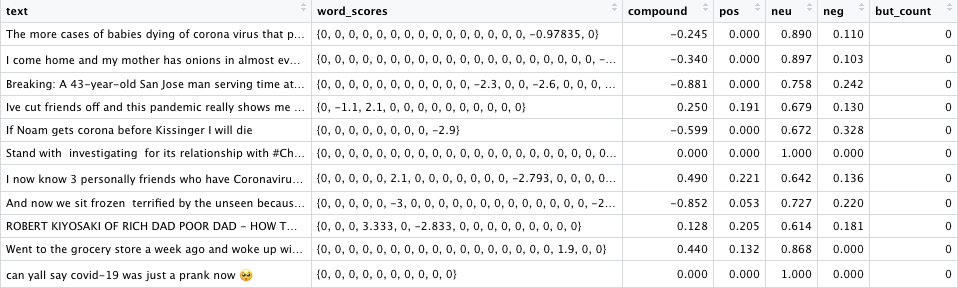
\includegraphics[width=\textwidth]{figs/vader-table.png}    
    \centering
    \caption{Example sentiment analysis output of VADER package.}
  \end{figure}
  \end{landscape}
%TC:endignore
\end{document}